\documentclass[1p]{elsarticle_modified}
%\bibliographystyle{elsarticle-num}

%\usepackage[colorlinks]{hyperref}
%\usepackage{abbrmath_seonhwa} %\Abb, \Ascr, \Acal ,\Abf, \Afrak
\usepackage{amsfonts}
\usepackage{amssymb}
\usepackage{amsmath}
\usepackage{amsthm}
\usepackage{scalefnt}
\usepackage{amsbsy}
\usepackage{kotex}
\usepackage{caption}
\usepackage{subfig}
\usepackage{color}
\usepackage{graphicx}
\usepackage{xcolor} %% white, black, red, green, blue, cyan, magenta, yellow
\usepackage{float}
\usepackage{setspace}
\usepackage{hyperref}

\usepackage{tikz}
\usetikzlibrary{arrows}

\usepackage{multirow}
\usepackage{array} % fixed length table
\usepackage{hhline}

%%%%%%%%%%%%%%%%%%%%%
\makeatletter
\renewcommand*\env@matrix[1][\arraystretch]{%
	\edef\arraystretch{#1}%
	\hskip -\arraycolsep
	\let\@ifnextchar\new@ifnextchar
	\array{*\c@MaxMatrixCols c}}
\makeatother %https://tex.stackexchange.com/questions/14071/how-can-i-increase-the-line-spacing-in-a-matrix
%%%%%%%%%%%%%%%

\usepackage[normalem]{ulem}

\newcommand{\msout}[1]{\ifmmode\text{\sout{\ensuremath{#1}}}\else\sout{#1}\fi}
%SOURCE: \msout is \stkout macro in https://tex.stackexchange.com/questions/20609/strikeout-in-math-mode

\newcommand{\cancel}[1]{
	\ifmmode
	{\color{red}\msout{#1}}
	\else
	{\color{red}\sout{#1}}
	\fi
}

\newcommand{\add}[1]{
	{\color{blue}\uwave{#1}}
}

\newcommand{\replace}[2]{
	\ifmmode
	{\color{red}\msout{#1}}{\color{blue}\uwave{#2}}
	\else
	{\color{red}\sout{#1}}{\color{blue}\uwave{#2}}
	\fi
}

\newcommand{\Sol}{\mathcal{S}} %segment
\newcommand{\D}{D} %diagram
\newcommand{\A}{\mathcal{A}} %arc


%%%%%%%%%%%%%%%%%%%%%%%%%%%%%5 test

\def\sl{\operatorname{\textup{SL}}(2,\Cbb)}
\def\psl{\operatorname{\textup{PSL}}(2,\Cbb)}
\def\quan{\mkern 1mu \triangleright \mkern 1mu}

\theoremstyle{definition}
\newtheorem{thm}{Theorem}[section]
\newtheorem{prop}[thm]{Proposition}
\newtheorem{lem}[thm]{Lemma}
\newtheorem{ques}[thm]{Question}
\newtheorem{cor}[thm]{Corollary}
\newtheorem{defn}[thm]{Definition}
\newtheorem{exam}[thm]{Example}
\newtheorem{rmk}[thm]{Remark}
\newtheorem{alg}[thm]{Algorithm}

\newcommand{\I}{\sqrt{-1}}
\begin{document}

%\begin{frontmatter}
%
%\title{Boundary parabolic representations of knots up to 8 crossings}
%
%%% Group authors per affiliation:
%\author{Yunhi Cho} 
%\address{Department of Mathematics, University of Seoul, Seoul, Korea}
%\ead{yhcho@uos.ac.kr}
%
%
%\author{Seonhwa Kim} %\fnref{s_kim}}
%\address{Center for Geometry and Physics, Institute for Basic Science, Pohang, 37673, Korea}
%\ead{ryeona17@ibs.re.kr}
%
%\author{Hyuk Kim}
%\address{Department of Mathematical Sciences, Seoul National University, Seoul 08826, Korea}
%\ead{hyukkim@snu.ac.kr}
%
%\author{Seokbeom Yoon}
%\address{Department of Mathematical Sciences, Seoul National University, Seoul, 08826,  Korea}
%\ead{sbyoon15@snu.ac.kr}
%
%\begin{abstract}
%We find all boundary parabolic representation of knots up to 8 crossings.
%
%\end{abstract}
%\begin{keyword}
%    \MSC[2010] 57M25 
%\end{keyword}
%
%\end{frontmatter}

%\linenumbers
%\tableofcontents
%
\newcommand\colored[1]{\textcolor{white}{\rule[-0.35ex]{0.8em}{1.4ex}}\kern-0.8em\color{red} #1}%
%\newcommand\colored[1]{\textcolor{white}{ #1}\kern-2.17ex	\textcolor{white}{ #1}\kern-1.81ex	\textcolor{white}{ #1}\kern-2.15ex\color{red}#1	}

{\Large $\underline{12a_{1217}~(K12a_{1217})}$}

\setlength{\tabcolsep}{10pt}
\renewcommand{\arraystretch}{1.6}
\vspace{1cm}\begin{tabular}{m{100pt}>{\centering\arraybackslash}m{274pt}}
\multirow{5}{120pt}{
	\centering
	\includegraphics[width=112pt]{../../../GIT/diagram.site/Diagrams/png/2018_12a_1217.png}\\
\ \ \ A knot diagram\footnotemark}&
\allowdisplaybreaks
\textbf{Linearized knot diagam} \\
\cline{2-2}
 &
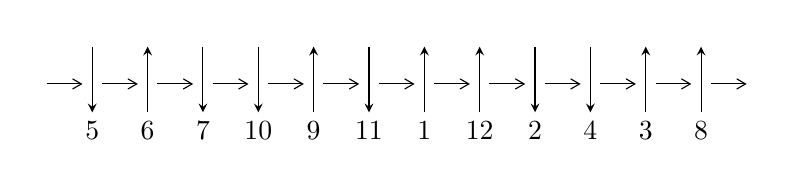
\begin{tikzpicture}[x=20pt, y=17pt]
	% nodes
	\node (C0) at (0, 0) {};
	\node (C1) at (1, 0) {};
	\node (C1U) at (1, +1) {};
	\node (C1D) at (1, -1) {5};

	\node (C2) at (2, 0) {};
	\node (C2U) at (2, +1) {};
	\node (C2D) at (2, -1) {6};

	\node (C3) at (3, 0) {};
	\node (C3U) at (3, +1) {};
	\node (C3D) at (3, -1) {7};

	\node (C4) at (4, 0) {};
	\node (C4U) at (4, +1) {};
	\node (C4D) at (4, -1) {10};

	\node (C5) at (5, 0) {};
	\node (C5U) at (5, +1) {};
	\node (C5D) at (5, -1) {9};

	\node (C6) at (6, 0) {};
	\node (C6U) at (6, +1) {};
	\node (C6D) at (6, -1) {11};

	\node (C7) at (7, 0) {};
	\node (C7U) at (7, +1) {};
	\node (C7D) at (7, -1) {1};

	\node (C8) at (8, 0) {};
	\node (C8U) at (8, +1) {};
	\node (C8D) at (8, -1) {12};

	\node (C9) at (9, 0) {};
	\node (C9U) at (9, +1) {};
	\node (C9D) at (9, -1) {2};

	\node (C10) at (10, 0) {};
	\node (C10U) at (10, +1) {};
	\node (C10D) at (10, -1) {4};

	\node (C11) at (11, 0) {};
	\node (C11U) at (11, +1) {};
	\node (C11D) at (11, -1) {3};

	\node (C12) at (12, 0) {};
	\node (C12U) at (12, +1) {};
	\node (C12D) at (12, -1) {8};
	\node (C13) at (13, 0) {};

	% arrows
	\draw[->,>={angle 60}]
	(C0) edge (C1) (C1) edge (C2) (C2) edge (C3) (C3) edge (C4) (C4) edge (C5) (C5) edge (C6) (C6) edge (C7) (C7) edge (C8) (C8) edge (C9) (C9) edge (C10) (C10) edge (C11) (C11) edge (C12) (C12) edge (C13) ;	\draw[->,>=stealth]
	(C1U) edge (C1D) (C2D) edge (C2U) (C3U) edge (C3D) (C4U) edge (C4D) (C5D) edge (C5U) (C6U) edge (C6D) (C7D) edge (C7U) (C8D) edge (C8U) (C9U) edge (C9D) (C10U) edge (C10D) (C11D) edge (C11U) (C12D) edge (C12U) ;
	\end{tikzpicture} \\
\hhline{~~} \\& 
\textbf{Solving Sequence} \\ \cline{2-2} 
 &
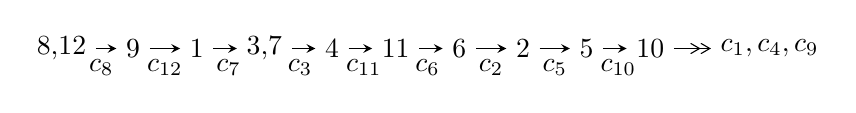
\begin{tikzpicture}[x=23pt, y=7pt]
	% node
	\node (A0) at (-1/8, 0) {8,12};
	\node (A1) at (1, 0) {9};
	\node (A2) at (2, 0) {1};
	\node (A3) at (49/16, 0) {3,7};
	\node (A4) at (33/8, 0) {4};
	\node (A5) at (41/8, 0) {11};
	\node (A6) at (49/8, 0) {6};
	\node (A7) at (57/8, 0) {2};
	\node (A8) at (65/8, 0) {5};
	\node (A9) at (73/8, 0) {10};
	\node (C1) at (1/2, -1) {$c_{8}$};
	\node (C2) at (3/2, -1) {$c_{12}$};
	\node (C3) at (5/2, -1) {$c_{7}$};
	\node (C4) at (29/8, -1) {$c_{3}$};
	\node (C5) at (37/8, -1) {$c_{11}$};
	\node (C6) at (45/8, -1) {$c_{6}$};
	\node (C7) at (53/8, -1) {$c_{2}$};
	\node (C8) at (61/8, -1) {$c_{5}$};
	\node (C9) at (69/8, -1) {$c_{10}$};
	\node (A10) at (11, 0) {$c_{1},c_{4},c_{9}$};

	% edge
	\draw[->,>=stealth]	
	(A0) edge (A1) (A1) edge (A2) (A2) edge (A3) (A3) edge (A4) (A4) edge (A5) (A5) edge (A6) (A6) edge (A7) (A7) edge (A8) (A8) edge (A9) ;
	\draw[->>,>={angle 60}]	
	(A9) edge (A10);
\end{tikzpicture} \\ 

\end{tabular} \\

\footnotetext{
The image of knot diagram is generated by the software ``\textbf{Draw programme}" developed by Andrew Bartholomew(\url{http://www.layer8.co.uk/maths/draw/index.htm\#Running-draw}), where we modified some parts for our purpose(\url{https://github.com/CATsTAILs/LinksPainter}).
}\phantom \\ \newline 
\centering \textbf{Ideals for irreducible components\footnotemark of $X_{\text{par}}$} 
 
\begin{align*}
I^u_{1}&=\langle 
-3.78483\times10^{62} u^{51}-9.23708\times10^{62} u^{50}+\cdots+3.66721\times10^{63} b-9.19913\times10^{63},\\
\phantom{I^u_{1}}&\phantom{= \langle  }-1.19194\times10^{64} u^{51}-3.36347\times10^{64} u^{50}+\cdots+1.02682\times10^{65} a-4.62060\times10^{65},\\
\phantom{I^u_{1}}&\phantom{= \langle  }u^{52}+3 u^{51}+\cdots+155 u+28\rangle \\
I^u_{2}&=\langle 
-6.32395\times10^{29} a u^{49}-6.85959\times10^{30} u^{49}+\cdots+4.20919\times10^{31} a-4.89805\times10^{31},\\
\phantom{I^u_{2}}&\phantom{= \langle  }5.23973\times10^{32} a u^{49}-4.49244\times10^{32} u^{49}+\cdots+4.28747\times10^{33} a+1.58434\times10^{33},\\
\phantom{I^u_{2}}&\phantom{= \langle  }u^{50}-2 u^{49}+\cdots-60 u+19\rangle \\
I^u_{3}&=\langle 
u^{12} a+u^{12}+\cdots- a+11,\;34 u^{12} a+40 u^{12}+\cdots+85 a+269,\\
\phantom{I^u_{3}}&\phantom{= \langle  }u^{13}-2 u^{12}+9 u^{11}-15 u^{10}+32 u^9-45 u^8+58 u^7-66 u^6+55 u^5-44 u^4+24 u^3-8 u^2+3 u+1\rangle \\
I^u_{4}&=\langle 
u^7+3 u^6+7 u^5+10 u^4+11 u^3+8 u^2+b+4 u+1,\;u^6+2 u^5+5 u^4+6 u^3+7 u^2+a+4 u+3,\\
\phantom{I^u_{4}}&\phantom{= \langle  }u^8+2 u^7+6 u^6+8 u^5+11 u^4+9 u^3+7 u^2+2 u+1\rangle \\
\\
\end{align*}
\raggedright * 4 irreducible components of $\dim_{\mathbb{C}}=0$, with total 186 representations.\\
\footnotetext{All coefficients of polynomials are rational numbers. But the coefficients are sometimes approximated in decimal forms when there is not enough margin.}
\newpage
\renewcommand{\arraystretch}{1}
\centering \section*{I. $I^u_{1}= \langle -3.78\times10^{62} u^{51}-9.24\times10^{62} u^{50}+\cdots+3.67\times10^{63} b-9.20\times10^{63},\;-1.19\times10^{64} u^{51}-3.36\times10^{64} u^{50}+\cdots+1.03\times10^{65} a-4.62\times10^{65},\;u^{52}+3 u^{51}+\cdots+155 u+28 \rangle$}
\flushleft \textbf{(i) Arc colorings}\\
\begin{tabular}{m{7pt} m{180pt} m{7pt} m{180pt} }
\flushright $a_{8}=$&$\begin{pmatrix}1\\0\end{pmatrix}$ \\
\flushright $a_{12}=$&$\begin{pmatrix}0\\u\end{pmatrix}$ \\
\flushright $a_{9}=$&$\begin{pmatrix}1\\- u^2\end{pmatrix}$ \\
\flushright $a_{1}=$&$\begin{pmatrix}u\\u\end{pmatrix}$ \\
\flushright $a_{3}=$&$\begin{pmatrix}0.116080 u^{51}+0.327562 u^{50}+\cdots+24.4948 u+4.49991\\0.103207 u^{51}+0.251883 u^{50}+\cdots+11.1540 u+2.50848\end{pmatrix}$ \\
\flushright $a_{7}=$&$\begin{pmatrix}u^2+1\\u^2\end{pmatrix}$ \\
\flushright $a_{4}=$&$\begin{pmatrix}0.102816 u^{51}+0.276430 u^{50}+\cdots+12.5832 u+1.52396\\0.168183 u^{51}+0.455833 u^{50}+\cdots+16.5012 u+3.07868\end{pmatrix}$ \\
\flushright $a_{11}=$&$\begin{pmatrix}-0.0592969 u^{51}-0.158117 u^{50}+\cdots-23.0526 u-8.06748\\-0.0168503 u^{51}-0.0486054 u^{50}+\cdots-3.42539 u-2.09057\end{pmatrix}$ \\
\flushright $a_{6}=$&$\begin{pmatrix}-0.110268 u^{51}-0.272050 u^{50}+\cdots-30.8258 u-5.98247\\0.0385349 u^{51}+0.0641253 u^{50}+\cdots-7.47331 u-1.60516\end{pmatrix}$ \\
\flushright $a_{2}=$&$\begin{pmatrix}-0.264232 u^{51}-0.613333 u^{50}+\cdots-41.2535 u-8.42966\\0.0828615 u^{51}+0.241500 u^{50}+\cdots+18.5521 u+3.43075\end{pmatrix}$ \\
\flushright $a_{5}=$&$\begin{pmatrix}-0.0895885 u^{51}-0.165558 u^{50}+\cdots-17.3333 u-2.73222\\0.0370596 u^{51}+0.136146 u^{50}+\cdots-0.00391984 u-0.360451\end{pmatrix}$ \\
\flushright $a_{10}=$&$\begin{pmatrix}-0.156030 u^{51}-0.415662 u^{50}+\cdots-41.1156 u-8.35564\\0.0842371 u^{51}+0.0643931 u^{50}+\cdots-1.68892 u-0.0133933\end{pmatrix}$\\&\end{tabular}
\flushleft \textbf{(ii) Obstruction class $= -1$}\\~\\
\flushleft \textbf{(iii) Cusp Shapes $= -0.236976 u^{51}-0.873090 u^{50}+\cdots-17.6537 u-4.16045$}\\~\\
\newpage\renewcommand{\arraystretch}{1}
\flushleft \textbf{(iv) u-Polynomials at the component}\newline \\
\begin{tabular}{m{50pt}|m{274pt}}
Crossings & \hspace{64pt}u-Polynomials at each crossing \\
\hline $$\begin{aligned}c_{1},c_{3}\end{aligned}$$&$\begin{aligned}
&u^{52}-3 u^{51}+\cdots-1044 u+68
\end{aligned}$\\
\hline $$\begin{aligned}c_{2}\end{aligned}$$&$\begin{aligned}
&u^{52}-8 u^{51}+\cdots-50175 u+6372
\end{aligned}$\\
\hline $$\begin{aligned}c_{4},c_{10}\end{aligned}$$&$\begin{aligned}
&17(17 u^{52}+9 u^{51}+\cdots-1024 u+512)
\end{aligned}$\\
\hline $$\begin{aligned}c_{5},c_{11}\end{aligned}$$&$\begin{aligned}
&17(17 u^{52}+43 u^{51}+\cdots+9 u+1)
\end{aligned}$\\
\hline $$\begin{aligned}c_{6},c_{9}\end{aligned}$$&$\begin{aligned}
&u^{52}+6 u^{50}+\cdots+94 u+17
\end{aligned}$\\
\hline $$\begin{aligned}c_{7},c_{8},c_{12}\end{aligned}$$&$\begin{aligned}
&u^{52}-3 u^{51}+\cdots-155 u+28
\end{aligned}$\\
\hline
\end{tabular}\\~\\
\newpage\renewcommand{\arraystretch}{1}
\flushleft \textbf{(v) Riley Polynomials at the component}\newline \\
\begin{tabular}{m{50pt}|m{274pt}}
Crossings & \hspace{64pt}Riley Polynomials at each crossing \\
\hline $$\begin{aligned}c_{1},c_{3}\end{aligned}$$&$\begin{aligned}
&y^{52}+y^{51}+\cdots-78640 y+4624
\end{aligned}$\\
\hline $$\begin{aligned}c_{2}\end{aligned}$$&$\begin{aligned}
&y^{52}+8 y^{51}+\cdots-699178473 y+40602384
\end{aligned}$\\
\hline $$\begin{aligned}c_{4},c_{10}\end{aligned}$$&$\begin{aligned}
&289(289 y^{52}+10289 y^{51}+\cdots-393216 y+262144)
\end{aligned}$\\
\hline $$\begin{aligned}c_{5},c_{11}\end{aligned}$$&$\begin{aligned}
&289(289 y^{52}+3931 y^{51}+\cdots+49 y+1)
\end{aligned}$\\
\hline $$\begin{aligned}c_{6},c_{9}\end{aligned}$$&$\begin{aligned}
&y^{52}+12 y^{51}+\cdots-3464 y+289
\end{aligned}$\\
\hline $$\begin{aligned}c_{7},c_{8},c_{12}\end{aligned}$$&$\begin{aligned}
&y^{52}+45 y^{51}+\cdots-6105 y+784
\end{aligned}$\\
\hline
\end{tabular}\\~\\
\newpage\flushleft \textbf{(vi) Complex Volumes and Cusp Shapes}
$$\begin{array}{c|c|c}  
\text{Solutions to }I^u_{1}& \I (\text{vol} + \sqrt{-1}CS) & \text{Cusp shape}\\
 \hline 
\begin{aligned}
u &= -0.950344 + 0.322119 I \\
a &= \phantom{-}1.36230 - 0.69032 I \\
b &= \phantom{-}0.884105 + 0.214283 I\end{aligned}
 & \phantom{-}6.7763 - 15.3902 I & \phantom{-}3.50991 + 9.23358 I \\ \hline\begin{aligned}
u &= -0.950344 - 0.322119 I \\
a &= \phantom{-}1.36230 + 0.69032 I \\
b &= \phantom{-}0.884105 - 0.214283 I\end{aligned}
 & \phantom{-}6.7763 + 15.3902 I & \phantom{-}3.50991 - 9.23358 I \\ \hline\begin{aligned}
u &= \phantom{-}0.611986 + 0.823380 I \\
a &= \phantom{-}0.290031 + 0.143467 I \\
b &= -0.191685 + 0.783395 I\end{aligned}
 & \phantom{-}5.64694 + 2.40410 I & \phantom{-}6.40463 - 1.49639 I \\ \hline\begin{aligned}
u &= \phantom{-}0.611986 - 0.823380 I \\
a &= \phantom{-}0.290031 - 0.143467 I \\
b &= -0.191685 - 0.783395 I\end{aligned}
 & \phantom{-}5.64694 - 2.40410 I & \phantom{-}6.40463 + 1.49639 I \\ \hline\begin{aligned}
u &= -0.681639 + 0.820596 I \\
a &= -0.531183 + 0.353604 I \\
b &= -0.207357 + 0.308169 I\end{aligned}
 & \phantom{-}0.58300 - 2.55616 I & \phantom{-0.000000 } 0. - 10.37772 I \\ \hline\begin{aligned}
u &= -0.681639 - 0.820596 I \\
a &= -0.531183 - 0.353604 I \\
b &= -0.207357 - 0.308169 I\end{aligned}
 & \phantom{-}0.58300 + 2.55616 I & \phantom{-0.000000 -}0. + 10.37772 I \\ \hline\begin{aligned}
u &= \phantom{-}0.543343 + 0.739525 I \\
a &= -0.270104 - 1.316570 I \\
b &= -0.039019 - 0.651155 I\end{aligned}
 & -0.43165 - 5.19465 I & -2.45142 + 6.35490 I \\ \hline\begin{aligned}
u &= \phantom{-}0.543343 - 0.739525 I \\
a &= -0.270104 + 1.316570 I \\
b &= -0.039019 + 0.651155 I\end{aligned}
 & -0.43165 + 5.19465 I & -2.45142 - 6.35490 I \\ \hline\begin{aligned}
u &= -0.120480 + 1.099310 I \\
a &= -0.218284 - 0.770739 I \\
b &= \phantom{-}1.12128 - 0.86767 I\end{aligned}
 & \phantom{-}0.82652 - 6.20060 I & \phantom{-0.000000 -}0. + 7.06936 I \\ \hline\begin{aligned}
u &= -0.120480 - 1.099310 I \\
a &= -0.218284 + 0.770739 I \\
b &= \phantom{-}1.12128 + 0.86767 I\end{aligned}
 & \phantom{-}0.82652 + 6.20060 I & \phantom{-0.000000 } 0. - 7.06936 I\\
 \hline 
 \end{array}$$\newpage$$\begin{array}{c|c|c}  
\text{Solutions to }I^u_{1}& \I (\text{vol} + \sqrt{-1}CS) & \text{Cusp shape}\\
 \hline 
\begin{aligned}
u &= \phantom{-}0.766416 + 0.315534 I \\
a &= -1.80534 - 0.65677 I \\
b &= -0.925661 + 0.046111 I\end{aligned}
 & \phantom{-}0.92463 + 9.67458 I & \phantom{-}0.95373 - 10.15291 I \\ \hline\begin{aligned}
u &= \phantom{-}0.766416 - 0.315534 I \\
a &= -1.80534 + 0.65677 I \\
b &= -0.925661 - 0.046111 I\end{aligned}
 & \phantom{-}0.92463 - 9.67458 I & \phantom{-}0.95373 + 10.15291 I \\ \hline\begin{aligned}
u &= -0.784865 + 0.085590 I \\
a &= -0.781041 + 0.938598 I \\
b &= -0.373670 + 0.098029 I\end{aligned}
 & \phantom{-}2.02396 - 1.07247 I & \phantom{-}0.35961 + 2.83019 I \\ \hline\begin{aligned}
u &= -0.784865 - 0.085590 I \\
a &= -0.781041 - 0.938598 I \\
b &= -0.373670 - 0.098029 I\end{aligned}
 & \phantom{-}2.02396 + 1.07247 I & \phantom{-}0.35961 - 2.83019 I \\ \hline\begin{aligned}
u &= -0.089628 + 1.215000 I \\
a &= -0.506782 + 0.741949 I \\
b &= -1.62883 - 0.59977 I\end{aligned}
 & -0.06262 + 4.46410 I & \phantom{-0.000000 } 0 \\ \hline\begin{aligned}
u &= -0.089628 - 1.215000 I \\
a &= -0.506782 - 0.741949 I \\
b &= -1.62883 + 0.59977 I\end{aligned}
 & -0.06262 - 4.46410 I & \phantom{-0.000000 } 0 \\ \hline\begin{aligned}
u &= -0.727691 + 0.990444 I \\
a &= \phantom{-}0.248516 - 1.062610 I \\
b &= \phantom{-}0.408630 - 0.571110 I\end{aligned}
 & \phantom{-}4.83035 + 9.64704 I & \phantom{-0.000000 } 0 \\ \hline\begin{aligned}
u &= -0.727691 - 0.990444 I \\
a &= \phantom{-}0.248516 + 1.062610 I \\
b &= \phantom{-}0.408630 + 0.571110 I\end{aligned}
 & \phantom{-}4.83035 - 9.64704 I & \phantom{-0.000000 } 0 \\ \hline\begin{aligned}
u &= -0.248355 + 1.254680 I \\
a &= -0.424101 + 1.097270 I \\
b &= -0.12990 + 1.95024 I\end{aligned}
 & -1.52199 - 2.58358 I & \phantom{-0.000000 } 0 \\ \hline\begin{aligned}
u &= -0.248355 - 1.254680 I \\
a &= -0.424101 - 1.097270 I \\
b &= -0.12990 - 1.95024 I\end{aligned}
 & -1.52199 + 2.58358 I & \phantom{-0.000000 } 0\\
 \hline 
 \end{array}$$\newpage$$\begin{array}{c|c|c}  
\text{Solutions to }I^u_{1}& \I (\text{vol} + \sqrt{-1}CS) & \text{Cusp shape}\\
 \hline 
\begin{aligned}
u &= -0.596766 + 0.352197 I \\
a &= \phantom{-}0.061531 + 0.340342 I \\
b &= -0.775647 + 0.574721 I\end{aligned}
 & \phantom{-}2.70277 + 3.52281 I & -0.87054 - 2.02677 I \\ \hline\begin{aligned}
u &= -0.596766 - 0.352197 I \\
a &= \phantom{-}0.061531 - 0.340342 I \\
b &= -0.775647 - 0.574721 I\end{aligned}
 & \phantom{-}2.70277 - 3.52281 I & -0.87054 + 2.02677 I \\ \hline\begin{aligned}
u &= \phantom{-}1.037590 + 0.811762 I \\
a &= \phantom{-}0.531961 + 0.511091 I \\
b &= \phantom{-}0.475050 + 0.089805 I\end{aligned}
 & \phantom{-}3.22572 + 3.55521 I & \phantom{-0.000000 } 0 \\ \hline\begin{aligned}
u &= \phantom{-}1.037590 - 0.811762 I \\
a &= \phantom{-}0.531961 - 0.511091 I \\
b &= \phantom{-}0.475050 - 0.089805 I\end{aligned}
 & \phantom{-}3.22572 - 3.55521 I & \phantom{-0.000000 } 0 \\ \hline\begin{aligned}
u &= \phantom{-}0.558051 + 0.379501 I \\
a &= \phantom{-}1.164260 + 0.600486 I \\
b &= \phantom{-}0.547966 - 0.424737 I\end{aligned}
 & -1.36085 + 3.43390 I & -6.76914 - 8.21807 I \\ \hline\begin{aligned}
u &= \phantom{-}0.558051 - 0.379501 I \\
a &= \phantom{-}1.164260 - 0.600486 I \\
b &= \phantom{-}0.547966 + 0.424737 I\end{aligned}
 & -1.36085 - 3.43390 I & -6.76914 + 8.21807 I \\ \hline\begin{aligned}
u &= -0.122610 + 1.325890 I \\
a &= \phantom{-}0.708094 + 0.759028 I \\
b &= \phantom{-}2.33633 + 0.17751 I\end{aligned}
 & -1.84227 - 2.86744 I & \phantom{-0.000000 } 0 \\ \hline\begin{aligned}
u &= -0.122610 - 1.325890 I \\
a &= \phantom{-}0.708094 - 0.759028 I \\
b &= \phantom{-}2.33633 - 0.17751 I\end{aligned}
 & -1.84227 + 2.86744 I & \phantom{-0.000000 } 0 \\ \hline\begin{aligned}
u &= -0.549323 + 0.253198 I \\
a &= -1.21969 + 0.81806 I \\
b &= -0.465578 - 0.970504 I\end{aligned}
 & \phantom{-}2.63275 - 6.47736 I & -1.14133 + 11.11228 I \\ \hline\begin{aligned}
u &= -0.549323 - 0.253198 I \\
a &= -1.21969 - 0.81806 I \\
b &= -0.465578 + 0.970504 I\end{aligned}
 & \phantom{-}2.63275 + 6.47736 I & -1.14133 - 11.11228 I\\
 \hline 
 \end{array}$$\newpage$$\begin{array}{c|c|c}  
\text{Solutions to }I^u_{1}& \I (\text{vol} + \sqrt{-1}CS) & \text{Cusp shape}\\
 \hline 
\begin{aligned}
u &= -0.377950 + 1.358930 I \\
a &= \phantom{-}0.699285 + 0.212035 I \\
b &= \phantom{-}1.70671 - 0.17659 I\end{aligned}
 & -2.52853 - 5.35110 I & \phantom{-0.000000 } 0 \\ \hline\begin{aligned}
u &= -0.377950 - 1.358930 I \\
a &= \phantom{-}0.699285 - 0.212035 I \\
b &= \phantom{-}1.70671 + 0.17659 I\end{aligned}
 & -2.52853 + 5.35110 I & \phantom{-0.000000 } 0 \\ \hline\begin{aligned}
u &= \phantom{-}0.252344 + 1.391100 I \\
a &= -0.430609 + 0.154231 I \\
b &= -1.58256 - 0.68085 I\end{aligned}
 & -6.51872 + 2.69482 I & \phantom{-0.000000 } 0 \\ \hline\begin{aligned}
u &= \phantom{-}0.252344 - 1.391100 I \\
a &= -0.430609 - 0.154231 I \\
b &= -1.58256 + 0.68085 I\end{aligned}
 & -6.51872 - 2.69482 I & \phantom{-0.000000 } 0 \\ \hline\begin{aligned}
u &= -0.22905 + 1.40159 I \\
a &= \phantom{-}0.720518 + 0.079628 I \\
b &= \phantom{-}2.99526 + 0.53269 I\end{aligned}
 & -2.67681 - 9.40242 I & \phantom{-0.000000 } 0 \\ \hline\begin{aligned}
u &= -0.22905 - 1.40159 I \\
a &= \phantom{-}0.720518 - 0.079628 I \\
b &= \phantom{-}2.99526 - 0.53269 I\end{aligned}
 & -2.67681 + 9.40242 I & \phantom{-0.000000 } 0 \\ \hline\begin{aligned}
u &= -0.19045 + 1.43223 I \\
a &= \phantom{-}0.257532 + 0.194949 I \\
b &= \phantom{-}1.25353 - 0.98903 I\end{aligned}
 & -3.13364 + 0.73826 I & \phantom{-0.000000 } 0 \\ \hline\begin{aligned}
u &= -0.19045 - 1.43223 I \\
a &= \phantom{-}0.257532 - 0.194949 I \\
b &= \phantom{-}1.25353 + 0.98903 I\end{aligned}
 & -3.13364 - 0.73826 I & \phantom{-0.000000 } 0 \\ \hline\begin{aligned}
u &= \phantom{-}0.472544 + 0.263306 I \\
a &= \phantom{-}0.087356 + 0.662820 I \\
b &= \phantom{-}0.584757 + 0.218301 I\end{aligned}
 & -1.380760 - 0.242567 I & -6.94484 - 0.12994 I \\ \hline\begin{aligned}
u &= \phantom{-}0.472544 - 0.263306 I \\
a &= \phantom{-}0.087356 - 0.662820 I \\
b &= \phantom{-}0.584757 - 0.218301 I\end{aligned}
 & -1.380760 + 0.242567 I & -6.94484 + 0.12994 I\\
 \hline 
 \end{array}$$\newpage$$\begin{array}{c|c|c}  
\text{Solutions to }I^u_{1}& \I (\text{vol} + \sqrt{-1}CS) & \text{Cusp shape}\\
 \hline 
\begin{aligned}
u &= \phantom{-}0.20341 + 1.44904 I \\
a &= -0.755410 + 0.149534 I \\
b &= -2.69872 + 0.20686 I\end{aligned}
 & -7.26378 + 6.23517 I & \phantom{-0.000000 } 0 \\ \hline\begin{aligned}
u &= \phantom{-}0.20341 - 1.44904 I \\
a &= -0.755410 - 0.149534 I \\
b &= -2.69872 - 0.20686 I\end{aligned}
 & -7.26378 - 6.23517 I & \phantom{-0.000000 } 0 \\ \hline\begin{aligned}
u &= \phantom{-}0.30298 + 1.43159 I \\
a &= \phantom{-}1.052730 - 0.687104 I \\
b &= \phantom{-}3.01855 - 0.49877 I\end{aligned}
 & -4.6504 + 13.5551 I & \phantom{-0.000000 } 0 \\ \hline\begin{aligned}
u &= \phantom{-}0.30298 - 1.43159 I \\
a &= \phantom{-}1.052730 + 0.687104 I \\
b &= \phantom{-}3.01855 + 0.49877 I\end{aligned}
 & -4.6504 - 13.5551 I & \phantom{-0.000000 } 0 \\ \hline\begin{aligned}
u &= \phantom{-}0.04590 + 1.51101 I \\
a &= \phantom{-}0.842968 + 0.263947 I \\
b &= \phantom{-}2.09013 + 0.76931 I\end{aligned}
 & -8.16490 - 3.52694 I & \phantom{-0.000000 } 0 \\ \hline\begin{aligned}
u &= \phantom{-}0.04590 - 1.51101 I \\
a &= \phantom{-}0.842968 - 0.263947 I \\
b &= \phantom{-}2.09013 - 0.76931 I\end{aligned}
 & -8.16490 + 3.52694 I & \phantom{-0.000000 } 0 \\ \hline\begin{aligned}
u &= -0.37967 + 1.46684 I \\
a &= -0.971631 - 0.548746 I \\
b &= -2.85141 - 0.36099 I\end{aligned}
 & \phantom{-}1.0712 - 20.1676 I & \phantom{-0.000000 } 0 \\ \hline\begin{aligned}
u &= -0.37967 - 1.46684 I \\
a &= -0.971631 + 0.548746 I \\
b &= -2.85141 + 0.36099 I\end{aligned}
 & \phantom{-}1.0712 + 20.1676 I & \phantom{-0.000000 } 0 \\ \hline\begin{aligned}
u &= -0.358104 + 0.224691 I \\
a &= -2.05195 + 1.47795 I \\
b &= -0.730995 + 0.426246 I\end{aligned}
 & \phantom{-}2.90602 - 1.02604 I & -2.45090 + 4.57830 I \\ \hline\begin{aligned}
u &= -0.358104 - 0.224691 I \\
a &= -2.05195 - 1.47795 I \\
b &= -0.730995 - 0.426246 I\end{aligned}
 & \phantom{-}2.90602 + 1.02604 I & -2.45090 - 4.57830 I\\
 \hline 
 \end{array}$$\newpage$$\begin{array}{c|c|c}  
\text{Solutions to }I^u_{1}& \I (\text{vol} + \sqrt{-1}CS) & \text{Cusp shape}\\
 \hline 
\begin{aligned}
u &= \phantom{-}0.11236 + 1.65989 I \\
a &= -0.746881 + 0.209388 I \\
b &= -2.02713 + 0.41841 I\end{aligned}
 & -5.77267 + 7.71312 I & \phantom{-0.000000 } 0 \\ \hline\begin{aligned}
u &= \phantom{-}0.11236 - 1.65989 I \\
a &= -0.746881 - 0.209388 I \\
b &= -2.02713 - 0.41841 I\end{aligned}
 & -5.77267 - 7.71312 I & \phantom{-0.000000 } 0\\
 \hline 
 \end{array}$$\newpage\newpage\renewcommand{\arraystretch}{1}
\centering \section*{II. $I^u_{2}= \langle -6.32\times10^{29} a u^{49}-6.86\times10^{30} u^{49}+\cdots+4.21\times10^{31} a-4.90\times10^{31},\;5.24\times10^{32} a u^{49}-4.49\times10^{32} u^{49}+\cdots+4.29\times10^{33} a+1.58\times10^{33},\;u^{50}-2 u^{49}+\cdots-60 u+19 \rangle$}
\flushleft \textbf{(i) Arc colorings}\\
\begin{tabular}{m{7pt} m{180pt} m{7pt} m{180pt} }
\flushright $a_{8}=$&$\begin{pmatrix}1\\0\end{pmatrix}$ \\
\flushright $a_{12}=$&$\begin{pmatrix}0\\u\end{pmatrix}$ \\
\flushright $a_{9}=$&$\begin{pmatrix}1\\- u^2\end{pmatrix}$ \\
\flushright $a_{1}=$&$\begin{pmatrix}u\\u\end{pmatrix}$ \\
\flushright $a_{3}=$&$\begin{pmatrix}a\\0.576750 a u^{49}+6.25601 u^{49}+\cdots-38.3882 a+44.6707\end{pmatrix}$ \\
\flushright $a_{7}=$&$\begin{pmatrix}u^2+1\\u^2\end{pmatrix}$ \\
\flushright $a_{4}=$&$\begin{pmatrix}-0.469262 a u^{49}-1.44273 u^{49}+\cdots+9.18875 a-26.6023\\-0.0309561 a u^{49}+1.81285 u^{49}+\cdots+3.21660 a+19.2108\end{pmatrix}$ \\
\flushright $a_{11}=$&$\begin{pmatrix}-0.962384 a u^{49}+0.264443 u^{49}+\cdots-25.1510 a+21.5640\\-1.42355 a u^{49}-1.05929 u^{49}+\cdots-20.1266 a+10.7323\end{pmatrix}$ \\
\flushright $a_{6}=$&$\begin{pmatrix}-2.02043 a u^{49}+0.397524 u^{49}+\cdots+4.02193 a+44.8952\\-3.77917 a u^{49}+0.173659 u^{49}+\cdots-10.9582 a+29.0254\end{pmatrix}$ \\
\flushright $a_{2}=$&$\begin{pmatrix}2.03999 a u^{49}-0.314324 u^{49}+\cdots+117.548 a+22.1600\\2.72020 a u^{49}+0.169295 u^{49}+\cdots+189.705 a+6.65237\end{pmatrix}$ \\
\flushright $a_{5}=$&$\begin{pmatrix}-2.02043 a u^{49}-0.564860 u^{49}+\cdots+4.02193 a+19.7442\\-3.77917 a u^{49}-0.461168 u^{49}+\cdots-10.9582 a+5.02442\end{pmatrix}$ \\
\flushright $a_{10}=$&$\begin{pmatrix}0.388513 a u^{49}-1.01109 u^{49}+\cdots+32.7453 a+20.5741\\-0.509271 a u^{49}+0.194193 u^{49}+\cdots+51.2128 a-27.4119\end{pmatrix}$\\&\end{tabular}
\flushleft \textbf{(ii) Obstruction class $= -1$}\\~\\
\flushleft \textbf{(iii) Cusp Shapes $= -10.2250 u^{49}+10.1462 u^{48}+\cdots+237.491 u-95.5175$}\\~\\
\newpage\renewcommand{\arraystretch}{1}
\flushleft \textbf{(iv) u-Polynomials at the component}\newline \\
\begin{tabular}{m{50pt}|m{274pt}}
Crossings & \hspace{64pt}u-Polynomials at each crossing \\
\hline $$\begin{aligned}c_{1},c_{3}\end{aligned}$$&$\begin{aligned}
&u^{100}+3 u^{99}+\cdots-2324 u+5732
\end{aligned}$\\
\hline $$\begin{aligned}c_{2}\end{aligned}$$&$\begin{aligned}
&(u^{50}+7 u^{49}+\cdots+843 u+121)^{2}
\end{aligned}$\\
\hline $$\begin{aligned}c_{4},c_{10}\end{aligned}$$&$\begin{aligned}
&(u^{50}+u^{49}+\cdots+14 u-109)^{2}
\end{aligned}$\\
\hline $$\begin{aligned}c_{5},c_{11}\end{aligned}$$&$\begin{aligned}
&u^{100}+2 u^{99}+\cdots+44 u+1
\end{aligned}$\\
\hline $$\begin{aligned}c_{6},c_{9}\end{aligned}$$&$\begin{aligned}
&u^{100}+2 u^{99}+\cdots-23154 u+5887
\end{aligned}$\\
\hline $$\begin{aligned}c_{7},c_{8},c_{12}\end{aligned}$$&$\begin{aligned}
&(u^{50}+2 u^{49}+\cdots+60 u+19)^{2}
\end{aligned}$\\
\hline
\end{tabular}\\~\\
\newpage\renewcommand{\arraystretch}{1}
\flushleft \textbf{(v) Riley Polynomials at the component}\newline \\
\begin{tabular}{m{50pt}|m{274pt}}
Crossings & \hspace{64pt}Riley Polynomials at each crossing \\
\hline $$\begin{aligned}c_{1},c_{3}\end{aligned}$$&$\begin{aligned}
&y^{100}+35 y^{99}+\cdots+1531073088 y+32855824
\end{aligned}$\\
\hline $$\begin{aligned}c_{2}\end{aligned}$$&$\begin{aligned}
&(y^{50}-31 y^{49}+\cdots-433801 y+14641)^{2}
\end{aligned}$\\
\hline $$\begin{aligned}c_{4},c_{10}\end{aligned}$$&$\begin{aligned}
&(y^{50}+39 y^{49}+\cdots-91756 y+11881)^{2}
\end{aligned}$\\
\hline $$\begin{aligned}c_{5},c_{11}\end{aligned}$$&$\begin{aligned}
&y^{100}-38 y^{99}+\cdots-242 y+1
\end{aligned}$\\
\hline $$\begin{aligned}c_{6},c_{9}\end{aligned}$$&$\begin{aligned}
&y^{100}+26 y^{99}+\cdots+1584012916 y+34656769
\end{aligned}$\\
\hline $$\begin{aligned}c_{7},c_{8},c_{12}\end{aligned}$$&$\begin{aligned}
&(y^{50}+48 y^{49}+\cdots-4094 y+361)^{2}
\end{aligned}$\\
\hline
\end{tabular}\\~\\
\newpage\flushleft \textbf{(vi) Complex Volumes and Cusp Shapes}
$$\begin{array}{c|c|c}  
\text{Solutions to }I^u_{2}& \I (\text{vol} + \sqrt{-1}CS) & \text{Cusp shape}\\
 \hline 
\begin{aligned}
u &= -0.853092 + 0.375766 I \\
a &= \phantom{-}0.463582 + 0.017365 I \\
b &= \phantom{-}0.431688 + 0.229001 I\end{aligned}
 & \phantom{-}1.39801 - 3.06602 I & \phantom{-}3.27179 + 10.84309 I \\ \hline\begin{aligned}
u &= -0.853092 + 0.375766 I \\
a &= -1.39240 + 0.72586 I \\
b &= -0.720065 + 0.095569 I\end{aligned}
 & \phantom{-}1.39801 - 3.06602 I & \phantom{-}3.27179 + 10.84309 I \\ \hline\begin{aligned}
u &= -0.853092 - 0.375766 I \\
a &= \phantom{-}0.463582 - 0.017365 I \\
b &= \phantom{-}0.431688 - 0.229001 I\end{aligned}
 & \phantom{-}1.39801 + 3.06602 I & \phantom{-}3.27179 - 10.84309 I \\ \hline\begin{aligned}
u &= -0.853092 - 0.375766 I \\
a &= -1.39240 - 0.72586 I \\
b &= -0.720065 - 0.095569 I\end{aligned}
 & \phantom{-}1.39801 + 3.06602 I & \phantom{-}3.27179 - 10.84309 I \\ \hline\begin{aligned}
u &= \phantom{-}0.044252 + 1.114680 I \\
a &= \phantom{-}1.183460 - 0.165449 I \\
b &= \phantom{-}4.34484 + 0.02560 I\end{aligned}
 & \phantom{-}5.20918 - 4.43480 I & \phantom{-}4.65491 + 2.25442 I \\ \hline\begin{aligned}
u &= \phantom{-}0.044252 + 1.114680 I \\
a &= -0.341028 - 1.172380 I \\
b &= -0.010640 - 0.375629 I\end{aligned}
 & \phantom{-}5.20918 - 4.43480 I & \phantom{-}4.65491 + 2.25442 I \\ \hline\begin{aligned}
u &= \phantom{-}0.044252 - 1.114680 I \\
a &= \phantom{-}1.183460 + 0.165449 I \\
b &= \phantom{-}4.34484 - 0.02560 I\end{aligned}
 & \phantom{-}5.20918 + 4.43480 I & \phantom{-}4.65491 - 2.25442 I \\ \hline\begin{aligned}
u &= \phantom{-}0.044252 - 1.114680 I \\
a &= -0.341028 + 1.172380 I \\
b &= -0.010640 + 0.375629 I\end{aligned}
 & \phantom{-}5.20918 + 4.43480 I & \phantom{-}4.65491 - 2.25442 I \\ \hline\begin{aligned}
u &= \phantom{-}1.142970 + 0.129346 I \\
a &= \phantom{-}1.153980 + 0.810410 I \\
b &= \phantom{-}1.068290 - 0.191524 I\end{aligned}
 & \phantom{-}4.30836 + 5.93955 I & \phantom{-0.000000 } 0. - 19.3318 I \\ \hline\begin{aligned}
u &= \phantom{-}1.142970 + 0.129346 I \\
a &= -0.317165 - 0.294089 I \\
b &= -0.197641 - 0.018529 I\end{aligned}
 & \phantom{-}4.30836 + 5.93955 I & \phantom{-0.000000 } 0. - 19.3318 I\\
 \hline 
 \end{array}$$\newpage$$\begin{array}{c|c|c}  
\text{Solutions to }I^u_{2}& \I (\text{vol} + \sqrt{-1}CS) & \text{Cusp shape}\\
 \hline 
\begin{aligned}
u &= \phantom{-}1.142970 - 0.129346 I \\
a &= \phantom{-}1.153980 - 0.810410 I \\
b &= \phantom{-}1.068290 + 0.191524 I\end{aligned}
 & \phantom{-}4.30836 - 5.93955 I & \phantom{-0.000000 -}0. + 19.3318 I \\ \hline\begin{aligned}
u &= \phantom{-}1.142970 - 0.129346 I \\
a &= -0.317165 + 0.294089 I \\
b &= -0.197641 + 0.018529 I\end{aligned}
 & \phantom{-}4.30836 - 5.93955 I & \phantom{-0.000000 -}0. + 19.3318 I \\ \hline\begin{aligned}
u &= -0.678868 + 0.459434 I \\
a &= \phantom{-}0.354346 + 0.922133 I \\
b &= -0.140136 + 0.662804 I\end{aligned}
 & \phantom{-}5.87358 + 2.21185 I & \phantom{-}8.08574 - 3.74028 I \\ \hline\begin{aligned}
u &= -0.678868 + 0.459434 I \\
a &= -0.43873 - 1.46624 I \\
b &= -0.687287 + 0.630136 I\end{aligned}
 & \phantom{-}5.87358 + 2.21185 I & \phantom{-}8.08574 - 3.74028 I \\ \hline\begin{aligned}
u &= -0.678868 - 0.459434 I \\
a &= \phantom{-}0.354346 - 0.922133 I \\
b &= -0.140136 - 0.662804 I\end{aligned}
 & \phantom{-}5.87358 - 2.21185 I & \phantom{-}8.08574 + 3.74028 I \\ \hline\begin{aligned}
u &= -0.678868 - 0.459434 I \\
a &= -0.43873 + 1.46624 I \\
b &= -0.687287 - 0.630136 I\end{aligned}
 & \phantom{-}5.87358 - 2.21185 I & \phantom{-}8.08574 + 3.74028 I \\ \hline\begin{aligned}
u &= -0.112980 + 0.786145 I \\
a &= \phantom{-}0.637797 + 0.810591 I \\
b &= \phantom{-}0.441663 + 0.645929 I\end{aligned}
 & -1.24215 - 2.05779 I & -5.13529 + 4.01837 I \\ \hline\begin{aligned}
u &= -0.112980 + 0.786145 I \\
a &= -0.861384 + 0.661693 I \\
b &= \phantom{-}0.108824 + 0.340962 I\end{aligned}
 & -1.24215 - 2.05779 I & -5.13529 + 4.01837 I \\ \hline\begin{aligned}
u &= -0.112980 - 0.786145 I \\
a &= \phantom{-}0.637797 - 0.810591 I \\
b &= \phantom{-}0.441663 - 0.645929 I\end{aligned}
 & -1.24215 + 2.05779 I & -5.13529 - 4.01837 I \\ \hline\begin{aligned}
u &= -0.112980 - 0.786145 I \\
a &= -0.861384 - 0.661693 I \\
b &= \phantom{-}0.108824 - 0.340962 I\end{aligned}
 & -1.24215 + 2.05779 I & -5.13529 - 4.01837 I\\
 \hline 
 \end{array}$$\newpage$$\begin{array}{c|c|c}  
\text{Solutions to }I^u_{2}& \I (\text{vol} + \sqrt{-1}CS) & \text{Cusp shape}\\
 \hline 
\begin{aligned}
u &= \phantom{-}0.005335 + 1.206560 I \\
a &= -0.406736 + 1.318270 I \\
b &= -0.59428 + 1.36940 I\end{aligned}
 & \phantom{-}4.38592 + 4.77177 I & \phantom{-0.000000 } 0 \\ \hline\begin{aligned}
u &= \phantom{-}0.005335 + 1.206560 I \\
a &= \phantom{-}0.0174261 + 0.0722519 I \\
b &= -4.73862 + 0.89005 I\end{aligned}
 & \phantom{-}4.38592 + 4.77177 I & \phantom{-0.000000 } 0 \\ \hline\begin{aligned}
u &= \phantom{-}0.005335 - 1.206560 I \\
a &= -0.406736 - 1.318270 I \\
b &= -0.59428 - 1.36940 I\end{aligned}
 & \phantom{-}4.38592 - 4.77177 I & \phantom{-0.000000 } 0 \\ \hline\begin{aligned}
u &= \phantom{-}0.005335 - 1.206560 I \\
a &= \phantom{-}0.0174261 - 0.0722519 I \\
b &= -4.73862 - 0.89005 I\end{aligned}
 & \phantom{-}4.38592 - 4.77177 I & \phantom{-0.000000 } 0 \\ \hline\begin{aligned}
u &= \phantom{-}0.125803 + 1.220000 I \\
a &= -0.003607 - 0.764728 I \\
b &= \phantom{-}0.146091 + 1.147280 I\end{aligned}
 & \phantom{-}2.80415 + 1.36558 I & \phantom{-0.000000 } 0 \\ \hline\begin{aligned}
u &= \phantom{-}0.125803 + 1.220000 I \\
a &= \phantom{-}0.222241 + 1.245950 I \\
b &= \phantom{-}0.74351 + 1.94444 I\end{aligned}
 & \phantom{-}2.80415 + 1.36558 I & \phantom{-0.000000 } 0 \\ \hline\begin{aligned}
u &= \phantom{-}0.125803 - 1.220000 I \\
a &= -0.003607 + 0.764728 I \\
b &= \phantom{-}0.146091 - 1.147280 I\end{aligned}
 & \phantom{-}2.80415 - 1.36558 I & \phantom{-0.000000 } 0 \\ \hline\begin{aligned}
u &= \phantom{-}0.125803 - 1.220000 I \\
a &= \phantom{-}0.222241 - 1.245950 I \\
b &= \phantom{-}0.74351 - 1.94444 I\end{aligned}
 & \phantom{-}2.80415 - 1.36558 I & \phantom{-0.000000 } 0 \\ \hline\begin{aligned}
u &= \phantom{-}0.048382 + 1.268830 I \\
a &= \phantom{-}0.248925 + 1.072820 I \\
b &= \phantom{-}0.329224 + 0.922712 I\end{aligned}
 & -1.59254 - 1.81613 I & \phantom{-0.000000 } 0 \\ \hline\begin{aligned}
u &= \phantom{-}0.048382 + 1.268830 I \\
a &= \phantom{-}0.0448583 + 0.1175780 I \\
b &= \phantom{-}1.54639 + 0.12552 I\end{aligned}
 & -1.59254 - 1.81613 I & \phantom{-0.000000 } 0\\
 \hline 
 \end{array}$$\newpage$$\begin{array}{c|c|c}  
\text{Solutions to }I^u_{2}& \I (\text{vol} + \sqrt{-1}CS) & \text{Cusp shape}\\
 \hline 
\begin{aligned}
u &= \phantom{-}0.048382 - 1.268830 I \\
a &= \phantom{-}0.248925 - 1.072820 I \\
b &= \phantom{-}0.329224 - 0.922712 I\end{aligned}
 & -1.59254 + 1.81613 I & \phantom{-0.000000 } 0 \\ \hline\begin{aligned}
u &= \phantom{-}0.048382 - 1.268830 I \\
a &= \phantom{-}0.0448583 - 0.1175780 I \\
b &= \phantom{-}1.54639 - 0.12552 I\end{aligned}
 & -1.59254 + 1.81613 I & \phantom{-0.000000 } 0 \\ \hline\begin{aligned}
u &= \phantom{-}0.670397 + 0.276080 I \\
a &= -1.76420 - 0.28526 I \\
b &= -0.917938 + 0.521667 I\end{aligned}
 & \phantom{-}7.01035 + 7.12560 I & \phantom{-}8.18906 - 7.44187 I \\ \hline\begin{aligned}
u &= \phantom{-}0.670397 + 0.276080 I \\
a &= -1.02274 + 2.04880 I \\
b &= -0.662347 - 0.212692 I\end{aligned}
 & \phantom{-}7.01035 + 7.12560 I & \phantom{-}8.18906 - 7.44187 I \\ \hline\begin{aligned}
u &= \phantom{-}0.670397 - 0.276080 I \\
a &= -1.76420 + 0.28526 I \\
b &= -0.917938 - 0.521667 I\end{aligned}
 & \phantom{-}7.01035 - 7.12560 I & \phantom{-}8.18906 + 7.44187 I \\ \hline\begin{aligned}
u &= \phantom{-}0.670397 - 0.276080 I \\
a &= -1.02274 - 2.04880 I \\
b &= -0.662347 + 0.212692 I\end{aligned}
 & \phantom{-}7.01035 - 7.12560 I & \phantom{-}8.18906 + 7.44187 I \\ \hline\begin{aligned}
u &= -0.617921 + 0.375337 I \\
a &= \phantom{-}1.009360 + 0.092506 I \\
b &= \phantom{-}1.77235 - 0.76889 I\end{aligned}
 & \phantom{-}5.94348 - 6.22168 I & \phantom{-}9.7112 + 10.3014 I \\ \hline\begin{aligned}
u &= -0.617921 + 0.375337 I \\
a &= -1.85217 + 0.38036 I \\
b &= -0.585915 - 0.406234 I\end{aligned}
 & \phantom{-}5.94348 - 6.22168 I & \phantom{-}9.7112 + 10.3014 I \\ \hline\begin{aligned}
u &= -0.617921 - 0.375337 I \\
a &= \phantom{-}1.009360 - 0.092506 I \\
b &= \phantom{-}1.77235 + 0.76889 I\end{aligned}
 & \phantom{-}5.94348 + 6.22168 I & \phantom{-}9.7112 - 10.3014 I \\ \hline\begin{aligned}
u &= -0.617921 - 0.375337 I \\
a &= -1.85217 - 0.38036 I \\
b &= -0.585915 + 0.406234 I\end{aligned}
 & \phantom{-}5.94348 + 6.22168 I & \phantom{-}9.7112 - 10.3014 I\\
 \hline 
 \end{array}$$\newpage$$\begin{array}{c|c|c}  
\text{Solutions to }I^u_{2}& \I (\text{vol} + \sqrt{-1}CS) & \text{Cusp shape}\\
 \hline 
\begin{aligned}
u &= \phantom{-}0.526791 + 0.459769 I \\
a &= \phantom{-}0.84206 - 1.22209 I \\
b &= -0.061240 - 0.451389 I\end{aligned}
 & \phantom{-}6.14716 - 3.57703 I & \phantom{-}10.00737 + 1.70187 I \\ \hline\begin{aligned}
u &= \phantom{-}0.526791 + 0.459769 I \\
a &= \phantom{-}1.37409 - 0.61960 I \\
b &= \phantom{-}1.69522 + 0.95920 I\end{aligned}
 & \phantom{-}6.14716 - 3.57703 I & \phantom{-}10.00737 + 1.70187 I \\ \hline\begin{aligned}
u &= \phantom{-}0.526791 - 0.459769 I \\
a &= \phantom{-}0.84206 + 1.22209 I \\
b &= -0.061240 + 0.451389 I\end{aligned}
 & \phantom{-}6.14716 + 3.57703 I & \phantom{-}10.00737 - 1.70187 I \\ \hline\begin{aligned}
u &= \phantom{-}0.526791 - 0.459769 I \\
a &= \phantom{-}1.37409 + 0.61960 I \\
b &= \phantom{-}1.69522 - 0.95920 I\end{aligned}
 & \phantom{-}6.14716 + 3.57703 I & \phantom{-}10.00737 - 1.70187 I \\ \hline\begin{aligned}
u &= -0.174909 + 1.320300 I \\
a &= -0.907411 - 0.914447 I \\
b &= -3.37304 - 1.13903 I\end{aligned}
 & -2.73234 - 2.38787 I & \phantom{-0.000000 } 0 \\ \hline\begin{aligned}
u &= -0.174909 + 1.320300 I \\
a &= \phantom{-}0.10701 - 1.52004 I \\
b &= -0.65165 - 1.95690 I\end{aligned}
 & -2.73234 - 2.38787 I & \phantom{-0.000000 } 0 \\ \hline\begin{aligned}
u &= -0.174909 - 1.320300 I \\
a &= -0.907411 + 0.914447 I \\
b &= -3.37304 + 1.13903 I\end{aligned}
 & -2.73234 + 2.38787 I & \phantom{-0.000000 } 0 \\ \hline\begin{aligned}
u &= -0.174909 - 1.320300 I \\
a &= \phantom{-}0.10701 + 1.52004 I \\
b &= -0.65165 + 1.95690 I\end{aligned}
 & -2.73234 + 2.38787 I & \phantom{-0.000000 } 0 \\ \hline\begin{aligned}
u &= \phantom{-}0.181356 + 1.346230 I \\
a &= -1.116740 + 0.490263 I \\
b &= -3.37696 + 0.71430 I\end{aligned}
 & -2.78326 + 6.40427 I & \phantom{-0.000000 } 0 \\ \hline\begin{aligned}
u &= \phantom{-}0.181356 + 1.346230 I \\
a &= \phantom{-}0.276595 - 0.652660 I \\
b &= \phantom{-}0.551421 + 0.750472 I\end{aligned}
 & -2.78326 + 6.40427 I & \phantom{-0.000000 } 0\\
 \hline 
 \end{array}$$\newpage$$\begin{array}{c|c|c}  
\text{Solutions to }I^u_{2}& \I (\text{vol} + \sqrt{-1}CS) & \text{Cusp shape}\\
 \hline 
\begin{aligned}
u &= \phantom{-}0.181356 - 1.346230 I \\
a &= -1.116740 - 0.490263 I \\
b &= -3.37696 - 0.71430 I\end{aligned}
 & -2.78326 - 6.40427 I & \phantom{-0.000000 } 0 \\ \hline\begin{aligned}
u &= \phantom{-}0.181356 - 1.346230 I \\
a &= \phantom{-}0.276595 + 0.652660 I \\
b &= \phantom{-}0.551421 - 0.750472 I\end{aligned}
 & -2.78326 - 6.40427 I & \phantom{-0.000000 } 0 \\ \hline\begin{aligned}
u &= -0.483100 + 1.288460 I \\
a &= -0.461572 + 1.154570 I \\
b &= -0.318050 + 1.152110 I\end{aligned}
 & -0.94231 - 2.57657 I & \phantom{-0.000000 } 0 \\ \hline\begin{aligned}
u &= -0.483100 + 1.288460 I \\
a &= -0.0824832 + 0.0764807 I \\
b &= -0.382551 + 0.298574 I\end{aligned}
 & -0.94231 - 2.57657 I & \phantom{-0.000000 } 0 \\ \hline\begin{aligned}
u &= -0.483100 - 1.288460 I \\
a &= -0.461572 - 1.154570 I \\
b &= -0.318050 - 1.152110 I\end{aligned}
 & -0.94231 + 2.57657 I & \phantom{-0.000000 } 0 \\ \hline\begin{aligned}
u &= -0.483100 - 1.288460 I \\
a &= -0.0824832 - 0.0764807 I \\
b &= -0.382551 - 0.298574 I\end{aligned}
 & -0.94231 + 2.57657 I & \phantom{-0.000000 } 0 \\ \hline\begin{aligned}
u &= \phantom{-}0.219024 + 1.376470 I \\
a &= -1.163940 + 0.421303 I \\
b &= -2.69240 + 0.43625 I\end{aligned}
 & \phantom{-}0.90247 + 3.77376 I & \phantom{-0.000000 } 0 \\ \hline\begin{aligned}
u &= \phantom{-}0.219024 + 1.376470 I \\
a &= \phantom{-}0.276091 - 0.249385 I \\
b &= \phantom{-}2.78869 + 0.01106 I\end{aligned}
 & \phantom{-}0.90247 + 3.77376 I & \phantom{-0.000000 } 0 \\ \hline\begin{aligned}
u &= \phantom{-}0.219024 - 1.376470 I \\
a &= -1.163940 - 0.421303 I \\
b &= -2.69240 - 0.43625 I\end{aligned}
 & \phantom{-}0.90247 - 3.77376 I & \phantom{-0.000000 } 0 \\ \hline\begin{aligned}
u &= \phantom{-}0.219024 - 1.376470 I \\
a &= \phantom{-}0.276091 + 0.249385 I \\
b &= \phantom{-}2.78869 - 0.01106 I\end{aligned}
 & \phantom{-}0.90247 - 3.77376 I & \phantom{-0.000000 } 0\\
 \hline 
 \end{array}$$\newpage$$\begin{array}{c|c|c}  
\text{Solutions to }I^u_{2}& \I (\text{vol} + \sqrt{-1}CS) & \text{Cusp shape}\\
 \hline 
\begin{aligned}
u &= \phantom{-}0.545636 + 0.174349 I \\
a &= -1.033890 + 0.176796 I \\
b &= -1.11182 + 0.94368 I\end{aligned}
 & \phantom{-}5.88007 + 0.94320 I & \phantom{-}11.80952 - 4.74435 I \\ \hline\begin{aligned}
u &= \phantom{-}0.545636 + 0.174349 I \\
a &= \phantom{-}2.09585 + 1.00488 I \\
b &= \phantom{-}0.131818 - 0.052740 I\end{aligned}
 & \phantom{-}5.88007 + 0.94320 I & \phantom{-}11.80952 - 4.74435 I \\ \hline\begin{aligned}
u &= \phantom{-}0.545636 - 0.174349 I \\
a &= -1.033890 - 0.176796 I \\
b &= -1.11182 - 0.94368 I\end{aligned}
 & \phantom{-}5.88007 - 0.94320 I & \phantom{-}11.80952 + 4.74435 I \\ \hline\begin{aligned}
u &= \phantom{-}0.545636 - 0.174349 I \\
a &= \phantom{-}2.09585 - 1.00488 I \\
b &= \phantom{-}0.131818 + 0.052740 I\end{aligned}
 & \phantom{-}5.88007 - 0.94320 I & \phantom{-}11.80952 + 4.74435 I \\ \hline\begin{aligned}
u &= \phantom{-}0.27087 + 1.40747 I \\
a &= \phantom{-}0.742204 - 0.592227 I \\
b &= \phantom{-}2.91164 - 0.67398 I\end{aligned}
 & \phantom{-}1.64321 + 10.58060 I & \phantom{-0.000000 } 0 \\ \hline\begin{aligned}
u &= \phantom{-}0.27087 + 1.40747 I \\
a &= -0.59359 - 1.29306 I \\
b &= -0.95440 - 1.80716 I\end{aligned}
 & \phantom{-}1.64321 + 10.58060 I & \phantom{-0.000000 } 0 \\ \hline\begin{aligned}
u &= \phantom{-}0.27087 - 1.40747 I \\
a &= \phantom{-}0.742204 + 0.592227 I \\
b &= \phantom{-}2.91164 + 0.67398 I\end{aligned}
 & \phantom{-}1.64321 - 10.58060 I & \phantom{-0.000000 } 0 \\ \hline\begin{aligned}
u &= \phantom{-}0.27087 - 1.40747 I \\
a &= -0.59359 + 1.29306 I \\
b &= -0.95440 + 1.80716 I\end{aligned}
 & \phantom{-}1.64321 - 10.58060 I & \phantom{-0.000000 } 0 \\ \hline\begin{aligned}
u &= -0.24739 + 1.43867 I \\
a &= \phantom{-}0.988248 + 0.467520 I \\
b &= \phantom{-}3.00664 + 0.74404 I\end{aligned}
 & \phantom{-}0.15005 - 9.43660 I & \phantom{-0.000000 } 0 \\ \hline\begin{aligned}
u &= -0.24739 + 1.43867 I \\
a &= -0.169282 - 0.539428 I \\
b &= -0.83416 + 1.37577 I\end{aligned}
 & \phantom{-}0.15005 - 9.43660 I & \phantom{-0.000000 } 0\\
 \hline 
 \end{array}$$\newpage$$\begin{array}{c|c|c}  
\text{Solutions to }I^u_{2}& \I (\text{vol} + \sqrt{-1}CS) & \text{Cusp shape}\\
 \hline 
\begin{aligned}
u &= -0.24739 - 1.43867 I \\
a &= \phantom{-}0.988248 - 0.467520 I \\
b &= \phantom{-}3.00664 - 0.74404 I\end{aligned}
 & \phantom{-}0.15005 + 9.43660 I & \phantom{-0.000000 } 0 \\ \hline\begin{aligned}
u &= -0.24739 - 1.43867 I \\
a &= -0.169282 + 0.539428 I \\
b &= -0.83416 - 1.37577 I\end{aligned}
 & \phantom{-}0.15005 + 9.43660 I & \phantom{-0.000000 } 0 \\ \hline\begin{aligned}
u &= -0.05270 + 1.48053 I \\
a &= \phantom{-}0.943169 - 0.175611 I \\
b &= \phantom{-}2.41240 - 0.70289 I\end{aligned}
 & -8.39115 - 2.77998 I & \phantom{-0.000000 } 0 \\ \hline\begin{aligned}
u &= -0.05270 + 1.48053 I \\
a &= -0.650925 - 0.232981 I \\
b &= -2.29835 - 0.82686 I\end{aligned}
 & -8.39115 - 2.77998 I & \phantom{-0.000000 } 0 \\ \hline\begin{aligned}
u &= -0.05270 - 1.48053 I \\
a &= \phantom{-}0.943169 + 0.175611 I \\
b &= \phantom{-}2.41240 + 0.70289 I\end{aligned}
 & -8.39115 + 2.77998 I & \phantom{-0.000000 } 0 \\ \hline\begin{aligned}
u &= -0.05270 - 1.48053 I \\
a &= -0.650925 + 0.232981 I \\
b &= -2.29835 + 0.82686 I\end{aligned}
 & -8.39115 + 2.77998 I & \phantom{-0.000000 } 0 \\ \hline\begin{aligned}
u &= \phantom{-}0.509032 + 0.082967 I \\
a &= -1.241340 - 0.406845 I \\
b &= -0.733130 - 0.966411 I\end{aligned}
 & \phantom{-}1.77592 + 3.92629 I & \phantom{-}5.93998 - 7.39122 I \\ \hline\begin{aligned}
u &= \phantom{-}0.509032 + 0.082967 I \\
a &= \phantom{-}2.23928 + 1.54842 I \\
b &= \phantom{-}0.606279 - 0.373631 I\end{aligned}
 & \phantom{-}1.77592 + 3.92629 I & \phantom{-}5.93998 - 7.39122 I \\ \hline\begin{aligned}
u &= \phantom{-}0.509032 - 0.082967 I \\
a &= -1.241340 + 0.406845 I \\
b &= -0.733130 + 0.966411 I\end{aligned}
 & \phantom{-}1.77592 - 3.92629 I & \phantom{-}5.93998 + 7.39122 I \\ \hline\begin{aligned}
u &= \phantom{-}0.509032 - 0.082967 I \\
a &= \phantom{-}2.23928 - 1.54842 I \\
b &= \phantom{-}0.606279 + 0.373631 I\end{aligned}
 & \phantom{-}1.77592 - 3.92629 I & \phantom{-}5.93998 + 7.39122 I\\
 \hline 
 \end{array}$$\newpage$$\begin{array}{c|c|c}  
\text{Solutions to }I^u_{2}& \I (\text{vol} + \sqrt{-1}CS) & \text{Cusp shape}\\
 \hline 
\begin{aligned}
u &= -0.31394 + 1.45260 I \\
a &= \phantom{-}1.060920 + 0.562240 I \\
b &= \phantom{-}2.80199 + 0.37238 I\end{aligned}
 & -4.42525 - 7.21278 I & \phantom{-0.000000 } 0 \\ \hline\begin{aligned}
u &= -0.31394 + 1.45260 I \\
a &= -0.391186 - 0.309239 I \\
b &= -1.57316 - 0.08193 I\end{aligned}
 & -4.42525 - 7.21278 I & \phantom{-0.000000 } 0 \\ \hline\begin{aligned}
u &= -0.31394 - 1.45260 I \\
a &= \phantom{-}1.060920 - 0.562240 I \\
b &= \phantom{-}2.80199 - 0.37238 I\end{aligned}
 & -4.42525 + 7.21278 I & \phantom{-0.000000 } 0 \\ \hline\begin{aligned}
u &= -0.31394 - 1.45260 I \\
a &= -0.391186 + 0.309239 I \\
b &= -1.57316 + 0.08193 I\end{aligned}
 & -4.42525 + 7.21278 I & \phantom{-0.000000 } 0 \\ \hline\begin{aligned}
u &= \phantom{-}0.35794 + 1.44478 I \\
a &= \phantom{-}0.166068 + 0.890628 I \\
b &= \phantom{-}0.317764 - 0.036538 I\end{aligned}
 & -0.499183 - 0.060271 I & \phantom{-0.000000 } 0 \\ \hline\begin{aligned}
u &= \phantom{-}0.35794 + 1.44478 I \\
a &= -0.463721 + 0.167701 I \\
b &= -0.922676 + 0.152184 I\end{aligned}
 & -0.499183 - 0.060271 I & \phantom{-0.000000 } 0 \\ \hline\begin{aligned}
u &= \phantom{-}0.35794 - 1.44478 I \\
a &= \phantom{-}0.166068 - 0.890628 I \\
b &= \phantom{-}0.317764 + 0.036538 I\end{aligned}
 & -0.499183 + 0.060271 I & \phantom{-0.000000 } 0 \\ \hline\begin{aligned}
u &= \phantom{-}0.35794 - 1.44478 I \\
a &= -0.463721 - 0.167701 I \\
b &= -0.922676 - 0.152184 I\end{aligned}
 & -0.499183 + 0.060271 I & \phantom{-0.000000 } 0 \\ \hline\begin{aligned}
u &= \phantom{-}0.44541 + 1.43777 I \\
a &= -0.924400 + 0.519011 I \\
b &= -2.74553 + 0.12658 I\end{aligned}
 & -0.77358 + 11.45920 I & \phantom{-0.000000 } 0 \\ \hline\begin{aligned}
u &= \phantom{-}0.44541 + 1.43777 I \\
a &= \phantom{-}0.504235 - 0.292630 I \\
b &= \phantom{-}1.259920 - 0.160589 I\end{aligned}
 & -0.77358 + 11.45920 I & \phantom{-0.000000 } 0\\
 \hline 
 \end{array}$$\newpage$$\begin{array}{c|c|c}  
\text{Solutions to }I^u_{2}& \I (\text{vol} + \sqrt{-1}CS) & \text{Cusp shape}\\
 \hline 
\begin{aligned}
u &= \phantom{-}0.44541 - 1.43777 I \\
a &= -0.924400 - 0.519011 I \\
b &= -2.74553 - 0.12658 I\end{aligned}
 & -0.77358 - 11.45920 I & \phantom{-0.000000 } 0 \\ \hline\begin{aligned}
u &= \phantom{-}0.44541 - 1.43777 I \\
a &= \phantom{-}0.504235 + 0.292630 I \\
b &= \phantom{-}1.259920 + 0.160589 I\end{aligned}
 & -0.77358 - 11.45920 I & \phantom{-0.000000 } 0 \\ \hline\begin{aligned}
u &= -0.490689\phantom{ +0.000000I} \\
a &= \phantom{-}3.23420 + 1.30418 I \\
b &= \phantom{-}1.038740 - 0.216776 I\end{aligned}
 & \phantom{-}1.48420\phantom{ +0.000000I} & \phantom{-}3.80140\phantom{ +0.000000I} \\ \hline\begin{aligned}
u &= -0.490689\phantom{ +0.000000I} \\
a &= \phantom{-}3.23420 - 1.30418 I \\
b &= \phantom{-}1.038740 + 0.216776 I\end{aligned}
 & \phantom{-}1.48420\phantom{ +0.000000I} & \phantom{-}3.80140\phantom{ +0.000000I} \\ \hline\begin{aligned}
u &= -0.484703\phantom{ +0.000000I} \\
a &= -2.08878 + 0.14937 I \\
b &= -0.585405 + 0.408865 I\end{aligned}
 & \phantom{-}1.82789\phantom{ +0.000000I} & \phantom{-}6.46830\phantom{ +0.000000I} \\ \hline\begin{aligned}
u &= -0.484703\phantom{ +0.000000I} \\
a &= -2.08878 - 0.14937 I \\
b &= -0.585405 - 0.408865 I\end{aligned}
 & \phantom{-}1.82789\phantom{ +0.000000I} & \phantom{-}6.46830\phantom{ +0.000000I} \\ \hline\begin{aligned}
u &= -0.07060 + 1.57371 I \\
a &= -0.163936 + 0.993992 I \\
b &= -0.537368 + 0.431012 I\end{aligned}
 & -1.27490 - 1.07364 I & \phantom{-0.000000 } 0 \\ \hline\begin{aligned}
u &= -0.07060 + 1.57371 I \\
a &= \phantom{-}0.298943 + 0.086182 I \\
b &= \phantom{-}0.951356 - 0.070277 I\end{aligned}
 & -1.27490 - 1.07364 I & \phantom{-0.000000 } 0 \\ \hline\begin{aligned}
u &= -0.07060 - 1.57371 I \\
a &= -0.163936 - 0.993992 I \\
b &= -0.537368 - 0.431012 I\end{aligned}
 & -1.27490 + 1.07364 I & \phantom{-0.000000 } 0 \\ \hline\begin{aligned}
u &= -0.07060 - 1.57371 I \\
a &= \phantom{-}0.298943 - 0.086182 I \\
b &= \phantom{-}0.951356 + 0.070277 I\end{aligned}
 & -1.27490 + 1.07364 I & \phantom{-0.000000 } 0\\
 \hline 
 \end{array}$$\newpage\newpage\renewcommand{\arraystretch}{1}
\centering \section*{III. $I^u_{3}= \langle u^{12} a+u^{12}+\cdots- a+11,\;34 u^{12} a+40 u^{12}+\cdots+85 a+269,\;u^{13}-2 u^{12}+\cdots+3 u+1 \rangle$}
\flushleft \textbf{(i) Arc colorings}\\
\begin{tabular}{m{7pt} m{180pt} m{7pt} m{180pt} }
\flushright $a_{8}=$&$\begin{pmatrix}1\\0\end{pmatrix}$ \\
\flushright $a_{12}=$&$\begin{pmatrix}0\\u\end{pmatrix}$ \\
\flushright $a_{9}=$&$\begin{pmatrix}1\\- u^2\end{pmatrix}$ \\
\flushright $a_{1}=$&$\begin{pmatrix}u\\u\end{pmatrix}$ \\
\flushright $a_{3}=$&$\begin{pmatrix}a\\-\frac{1}{3} u^{12} a-\frac{1}{3} u^{12}+\cdots+\frac{1}{3} a-\frac{11}{3}\end{pmatrix}$ \\
\flushright $a_{7}=$&$\begin{pmatrix}u^2+1\\u^2\end{pmatrix}$ \\
\flushright $a_{4}=$&$\begin{pmatrix}\frac{1}{3} u^{12} a+\frac{1}{3} u^{12}+\cdots+\frac{2}{3} a+\frac{5}{3}\\\frac{1}{3} u^{12} a-\frac{2}{3} u^{12}+\cdots-\frac{1}{3} a-\frac{10}{3}\end{pmatrix}$ \\
\flushright $a_{11}=$&$\begin{pmatrix}- u^{11} a-\frac{5}{17} u^{12}+\cdots-2 a-\frac{40}{17}\\\frac{2}{3} u^{12} a+\frac{73}{51} u^{12}+\cdots-\frac{2}{3} a+\frac{74}{51}\end{pmatrix}$ \\
\flushright $a_{6}=$&$\begin{pmatrix}\frac{1}{3} u^{12} a-\frac{5}{3} u^{12}+\cdots-\frac{7}{3} a-\frac{22}{3}\\\frac{2}{3} u^{12} a-\frac{1}{3} u^{12}+\cdots+\frac{1}{3} a+\frac{7}{3}\end{pmatrix}$ \\
\flushright $a_{2}=$&$\begin{pmatrix}\frac{2}{3} u^{12} a+\frac{2}{3} u^{12}+\cdots+\frac{4}{3} a+\frac{16}{3}\\2 u^{11} a- u^{12}+\cdots+a-3\end{pmatrix}$ \\
\flushright $a_{5}=$&$\begin{pmatrix}\frac{1}{3} u^{12} a-\frac{5}{3} u^{12}+\cdots-\frac{7}{3} a-\frac{28}{3}\\\frac{2}{3} u^{12} a+\frac{2}{3} u^{12}+\cdots+\frac{1}{3} a+\frac{4}{3}\end{pmatrix}$ \\
\flushright $a_{10}=$&$\begin{pmatrix}- u^{11} a+2 u^{12}+\cdots+a+8\\u^{12} a-2 u^{12}+\cdots- a-3 u\end{pmatrix}$\\&\end{tabular}
\flushleft \textbf{(ii) Obstruction class $= 1$}\\~\\
\flushleft \textbf{(iii) Cusp Shapes $= -3 u^{12}+10 u^{11}-32 u^{10}+71 u^9-126 u^8+194 u^7-240 u^6+249 u^5-217 u^4+134 u^3-59 u^2+11 u+12$}\\~\\
\newpage\renewcommand{\arraystretch}{1}
\flushleft \textbf{(iv) u-Polynomials at the component}\newline \\
\begin{tabular}{m{50pt}|m{274pt}}
Crossings & \hspace{64pt}u-Polynomials at each crossing \\
\hline $$\begin{aligned}c_{1},c_{3}\end{aligned}$$&$\begin{aligned}
&u^{26}+2 u^{25}+\cdots+352 u^2+68
\end{aligned}$\\
\hline $$\begin{aligned}c_{2}\end{aligned}$$&$\begin{aligned}
&(u^{13}-8 u^{12}+\cdots+11 u+7)^{2}
\end{aligned}$\\
\hline $$\begin{aligned}c_{4},c_{10}\end{aligned}$$&$\begin{aligned}
&17(17 u^{26}+317 u^{24}+\cdots+75887 u^{2}+11131)
\end{aligned}$\\
\hline $$\begin{aligned}c_{5},c_{11}\end{aligned}$$&$\begin{aligned}
&17(17 u^{26}-51 u^{25}+\cdots-4 u+1)
\end{aligned}$\\
\hline $$\begin{aligned}c_{6},c_{9}\end{aligned}$$&$\begin{aligned}
&u^{26}-3 u^{25}+\cdots+113 u^2+17
\end{aligned}$\\
\hline $$\begin{aligned}c_{7},c_{8}\end{aligned}$$&$\begin{aligned}
&(u^{13}-2 u^{12}+\cdots+3 u+1)^{2}
\end{aligned}$\\
\hline $$\begin{aligned}c_{12}\end{aligned}$$&$\begin{aligned}
&(u^{13}+2 u^{12}+\cdots+3 u-1)^{2}
\end{aligned}$\\
\hline
\end{tabular}\\~\\
\newpage\renewcommand{\arraystretch}{1}
\flushleft \textbf{(v) Riley Polynomials at the component}\newline \\
\begin{tabular}{m{50pt}|m{274pt}}
Crossings & \hspace{64pt}Riley Polynomials at each crossing \\
\hline $$\begin{aligned}c_{1},c_{3}\end{aligned}$$&$\begin{aligned}
&y^{26}+16 y^{25}+\cdots+47872 y+4624
\end{aligned}$\\
\hline $$\begin{aligned}c_{2}\end{aligned}$$&$\begin{aligned}
&(y^{13}-8 y^{12}+\cdots+303 y-49)^{2}
\end{aligned}$\\
\hline $$\begin{aligned}c_{4},c_{10}\end{aligned}$$&$\begin{aligned}
&289(17 y^{13}+317 y^{12}+\cdots+75887 y+11131)^{2}
\end{aligned}$\\
\hline $$\begin{aligned}c_{5},c_{11}\end{aligned}$$&$\begin{aligned}
&289(289 y^{26}-3383 y^{25}+\cdots-12 y+1)
\end{aligned}$\\
\hline $$\begin{aligned}c_{6},c_{9}\end{aligned}$$&$\begin{aligned}
&y^{26}+5 y^{25}+\cdots+3842 y+289
\end{aligned}$\\
\hline $$\begin{aligned}c_{7},c_{8},c_{12}\end{aligned}$$&$\begin{aligned}
&(y^{13}+14 y^{12}+\cdots+25 y-1)^{2}
\end{aligned}$\\
\hline
\end{tabular}\\~\\
\newpage\flushleft \textbf{(vi) Complex Volumes and Cusp Shapes}
$$\begin{array}{c|c|c}  
\text{Solutions to }I^u_{3}& \I (\text{vol} + \sqrt{-1}CS) & \text{Cusp shape}\\
 \hline 
\begin{aligned}
u &= \phantom{-}0.908624 + 0.142085 I \\
a &= \phantom{-}1.27668 + 0.78464 I \\
b &= \phantom{-}0.956911 - 0.389604 I\end{aligned}
 & \phantom{-}4.49130 + 5.51584 I & \phantom{-}6.31451 - 2.47719 I \\ \hline\begin{aligned}
u &= \phantom{-}0.908624 + 0.142085 I \\
a &= -0.381290 + 0.003958 I \\
b &= -0.330401 - 0.431738 I\end{aligned}
 & \phantom{-}4.49130 + 5.51584 I & \phantom{-}6.31451 - 2.47719 I \\ \hline\begin{aligned}
u &= \phantom{-}0.908624 - 0.142085 I \\
a &= \phantom{-}1.27668 - 0.78464 I \\
b &= \phantom{-}0.956911 + 0.389604 I\end{aligned}
 & \phantom{-}4.49130 - 5.51584 I & \phantom{-}6.31451 + 2.47719 I \\ \hline\begin{aligned}
u &= \phantom{-}0.908624 - 0.142085 I \\
a &= -0.381290 - 0.003958 I \\
b &= -0.330401 + 0.431738 I\end{aligned}
 & \phantom{-}4.49130 - 5.51584 I & \phantom{-}6.31451 + 2.47719 I \\ \hline\begin{aligned}
u &= \phantom{-}0.011602 + 1.218530 I \\
a &= \phantom{-}0.346263 + 1.261500 I \\
b &= \phantom{-}0.302325 + 1.122330 I\end{aligned}
 & \phantom{-}4.08814 - 4.55288 I & -6.51388 - 1.38146 I \\ \hline\begin{aligned}
u &= \phantom{-}0.011602 + 1.218530 I \\
a &= \phantom{-}0.533525 - 0.196381 I \\
b &= \phantom{-}4.85984 + 0.38998 I\end{aligned}
 & \phantom{-}4.08814 - 4.55288 I & -6.51388 - 1.38146 I \\ \hline\begin{aligned}
u &= \phantom{-}0.011602 - 1.218530 I \\
a &= \phantom{-}0.346263 - 1.261500 I \\
b &= \phantom{-}0.302325 - 1.122330 I\end{aligned}
 & \phantom{-}4.08814 + 4.55288 I & -6.51388 + 1.38146 I \\ \hline\begin{aligned}
u &= \phantom{-}0.011602 - 1.218530 I \\
a &= \phantom{-}0.533525 + 0.196381 I \\
b &= \phantom{-}4.85984 - 0.38998 I\end{aligned}
 & \phantom{-}4.08814 + 4.55288 I & -6.51388 + 1.38146 I \\ \hline\begin{aligned}
u &= \phantom{-}0.087631 + 0.681880 I \\
a &= \phantom{-}0.648174 + 0.318711 I \\
b &= -2.42238 + 0.66316 I\end{aligned}
 & \phantom{-}6.21876 + 4.83799 I & \phantom{-}10.45135 - 6.26851 I \\ \hline\begin{aligned}
u &= \phantom{-}0.087631 + 0.681880 I \\
a &= \phantom{-}0.91097 - 1.54991 I \\
b &= \phantom{-}0.360359 - 0.591792 I\end{aligned}
 & \phantom{-}6.21876 + 4.83799 I & \phantom{-}10.45135 - 6.26851 I\\
 \hline 
 \end{array}$$\newpage$$\begin{array}{c|c|c}  
\text{Solutions to }I^u_{3}& \I (\text{vol} + \sqrt{-1}CS) & \text{Cusp shape}\\
 \hline 
\begin{aligned}
u &= \phantom{-}0.087631 - 0.681880 I \\
a &= \phantom{-}0.648174 - 0.318711 I \\
b &= -2.42238 - 0.66316 I\end{aligned}
 & \phantom{-}6.21876 - 4.83799 I & \phantom{-}10.45135 + 6.26851 I \\ \hline\begin{aligned}
u &= \phantom{-}0.087631 - 0.681880 I \\
a &= \phantom{-}0.91097 + 1.54991 I \\
b &= \phantom{-}0.360359 + 0.591792 I\end{aligned}
 & \phantom{-}6.21876 - 4.83799 I & \phantom{-}10.45135 + 6.26851 I \\ \hline\begin{aligned}
u &= -0.366787 + 1.313730 I \\
a &= -0.600079 + 1.161840 I \\
b &= -0.64225 + 1.51319 I\end{aligned}
 & -0.87585 - 2.29682 I & \phantom{-}2.24764 - 6.91415 I \\ \hline\begin{aligned}
u &= -0.366787 + 1.313730 I \\
a &= \phantom{-}0.295205 - 0.422005 I \\
b &= \phantom{-}0.483790 - 0.782453 I\end{aligned}
 & -0.87585 - 2.29682 I & \phantom{-}2.24764 - 6.91415 I \\ \hline\begin{aligned}
u &= -0.366787 - 1.313730 I \\
a &= -0.600079 - 1.161840 I \\
b &= -0.64225 - 1.51319 I\end{aligned}
 & -0.87585 + 2.29682 I & \phantom{-}2.24764 + 6.91415 I \\ \hline\begin{aligned}
u &= -0.366787 - 1.313730 I \\
a &= \phantom{-}0.295205 + 0.422005 I \\
b &= \phantom{-}0.483790 + 0.782453 I\end{aligned}
 & -0.87585 + 2.29682 I & \phantom{-}2.24764 + 6.91415 I \\ \hline\begin{aligned}
u &= \phantom{-}0.27490 + 1.40809 I \\
a &= -0.894460 + 0.429020 I \\
b &= -3.03409 + 0.54029 I\end{aligned}
 & -0.65452 + 9.44192 I & -2.27737 - 7.35211 I \\ \hline\begin{aligned}
u &= \phantom{-}0.27490 + 1.40809 I \\
a &= \phantom{-}0.001485 - 0.491007 I \\
b &= -0.164012 + 0.562372 I\end{aligned}
 & -0.65452 + 9.44192 I & -2.27737 - 7.35211 I \\ \hline\begin{aligned}
u &= \phantom{-}0.27490 - 1.40809 I \\
a &= -0.894460 - 0.429020 I \\
b &= -3.03409 - 0.54029 I\end{aligned}
 & -0.65452 - 9.44192 I & -2.27737 + 7.35211 I \\ \hline\begin{aligned}
u &= \phantom{-}0.27490 - 1.40809 I \\
a &= \phantom{-}0.001485 + 0.491007 I \\
b &= -0.164012 - 0.562372 I\end{aligned}
 & -0.65452 - 9.44192 I & -2.27737 + 7.35211 I\\
 \hline 
 \end{array}$$\newpage$$\begin{array}{c|c|c}  
\text{Solutions to }I^u_{3}& \I (\text{vol} + \sqrt{-1}CS) & \text{Cusp shape}\\
 \hline 
\begin{aligned}
u &= \phantom{-}0.17411 + 1.55291 I \\
a &= -0.059473 + 0.931053 I \\
b &= -0.361402 + 0.069098 I\end{aligned}
 & -1.090940 - 0.479706 I & -4.73923 - 1.66529 I \\ \hline\begin{aligned}
u &= \phantom{-}0.17411 + 1.55291 I \\
a &= -0.227461 + 0.160748 I \\
b &= -0.842787 - 0.023903 I\end{aligned}
 & -1.090940 - 0.479706 I & -4.73923 - 1.66529 I \\ \hline\begin{aligned}
u &= \phantom{-}0.17411 - 1.55291 I \\
a &= -0.059473 - 0.931053 I \\
b &= -0.361402 - 0.069098 I\end{aligned}
 & -1.090940 + 0.479706 I & -4.73923 + 1.66529 I \\ \hline\begin{aligned}
u &= \phantom{-}0.17411 - 1.55291 I \\
a &= -0.227461 - 0.160748 I \\
b &= -0.842787 + 0.023903 I\end{aligned}
 & -1.090940 + 0.479706 I & -4.73923 + 1.66529 I \\ \hline\begin{aligned}
u &= -0.180166\phantom{ +0.000000I} \\
a &= -4.84954 + 1.75128 I \\
b &= \phantom{-}0.334095 - 0.912061 I\end{aligned}
 & \phantom{-}5.25505\phantom{ +0.000000I} & \phantom{-}7.03400\phantom{ +0.000000I} \\ \hline\begin{aligned}
u &= -0.180166\phantom{ +0.000000I} \\
a &= -4.84954 - 1.75128 I \\
b &= \phantom{-}0.334095 + 0.912061 I\end{aligned}
 & \phantom{-}5.25505\phantom{ +0.000000I} & \phantom{-}7.03400\phantom{ +0.000000I}\\
 \hline 
 \end{array}$$\newpage\newpage\renewcommand{\arraystretch}{1}
\centering \section*{IV. $I^u_{4}= \langle u^7+3 u^6+\cdots+b+1,\;u^6+2 u^5+5 u^4+6 u^3+7 u^2+a+4 u+3,\;u^8+2 u^7+\cdots+2 u+1 \rangle$}
\flushleft \textbf{(i) Arc colorings}\\
\begin{tabular}{m{7pt} m{180pt} m{7pt} m{180pt} }
\flushright $a_{8}=$&$\begin{pmatrix}1\\0\end{pmatrix}$ \\
\flushright $a_{12}=$&$\begin{pmatrix}0\\u\end{pmatrix}$ \\
\flushright $a_{9}=$&$\begin{pmatrix}1\\- u^2\end{pmatrix}$ \\
\flushright $a_{1}=$&$\begin{pmatrix}u\\u\end{pmatrix}$ \\
\flushright $a_{3}=$&$\begin{pmatrix}- u^6-2 u^5-5 u^4-6 u^3-7 u^2-4 u-3\\- u^7-3 u^6-7 u^5-10 u^4-11 u^3-8 u^2-4 u-1\end{pmatrix}$ \\
\flushright $a_{7}=$&$\begin{pmatrix}u^2+1\\u^2\end{pmatrix}$ \\
\flushright $a_{4}=$&$\begin{pmatrix}u^7+u^6+3 u^5+u^4+u^3-2 u^2- u-2\\- u^6-3 u^5-6 u^4-8 u^3-7 u^2-4 u-1\end{pmatrix}$ \\
\flushright $a_{11}=$&$\begin{pmatrix}- u^7-2 u^6-6 u^5-7 u^4-9 u^3-5 u^2-3 u+1\\u^4+2 u^3+3 u^2+3 u+1\end{pmatrix}$ \\
\flushright $a_{6}=$&$\begin{pmatrix}- u^6-2 u^5-5 u^4-6 u^3-6 u^2-4 u-2\\- u^7-3 u^6-7 u^5-11 u^4-12 u^3-9 u^2-5 u-1\end{pmatrix}$ \\
\flushright $a_{2}=$&$\begin{pmatrix}- u^5-2 u^4-4 u^3-5 u^2-3 u-1\\u^7+2 u^6+4 u^5+5 u^4+4 u^3+2 u^2+2 u+1\end{pmatrix}$ \\
\flushright $a_{5}=$&$\begin{pmatrix}u^7+u^6+3 u^5+u^4+u^3-2 u^2- u-2\\- u^6-3 u^5-6 u^4-8 u^3-7 u^2-4 u-1\end{pmatrix}$ \\
\flushright $a_{10}=$&$\begin{pmatrix}- u^7-2 u^6-6 u^5-7 u^4-9 u^3-5 u^2-3 u+1\\u^4+2 u^3+3 u^2+3 u+1\end{pmatrix}$\\&\end{tabular}
\flushleft \textbf{(ii) Obstruction class $= 1$}\\~\\
\flushleft \textbf{(iii) Cusp Shapes $= -5 u^7-5 u^6-14 u^5-6 u^4+2 u^3+7 u^2+13 u+2$}\\~\\
\newpage\renewcommand{\arraystretch}{1}
\flushleft \textbf{(iv) u-Polynomials at the component}\newline \\
\begin{tabular}{m{50pt}|m{274pt}}
Crossings & \hspace{64pt}u-Polynomials at each crossing \\
\hline $$\begin{aligned}c_{1},c_{3}\end{aligned}$$&$\begin{aligned}
&u^8-3 u^7+6 u^6-9 u^5+12 u^4-11 u^3+8 u^2-4 u+1
\end{aligned}$\\
\hline $$\begin{aligned}c_{2}\end{aligned}$$&$\begin{aligned}
&u^8+5 u^7+13 u^6+20 u^5+22 u^4+18 u^3+12 u^2+5 u+1
\end{aligned}$\\
\hline $$\begin{aligned}c_{4},c_{10}\end{aligned}$$&$\begin{aligned}
&u^8
\end{aligned}$\\
\hline $$\begin{aligned}c_{5},c_{11}\end{aligned}$$&$\begin{aligned}
&u^8- u^7+2 u^6- u^5+2 u^4- u^3+2 u^2+1
\end{aligned}$\\
\hline $$\begin{aligned}c_{6},c_{9}\end{aligned}$$&$\begin{aligned}
&u^8+2 u^6+u^5+2 u^4+u^3+2 u^2+u+1
\end{aligned}$\\
\hline $$\begin{aligned}c_{7},c_{8}\end{aligned}$$&$\begin{aligned}
&u^8+2 u^7+6 u^6+8 u^5+11 u^4+9 u^3+7 u^2+2 u+1
\end{aligned}$\\
\hline $$\begin{aligned}c_{12}\end{aligned}$$&$\begin{aligned}
&u^8-2 u^7+6 u^6-8 u^5+11 u^4-9 u^3+7 u^2-2 u+1
\end{aligned}$\\
\hline
\end{tabular}\\~\\
\newpage\renewcommand{\arraystretch}{1}
\flushleft \textbf{(v) Riley Polynomials at the component}\newline \\
\begin{tabular}{m{50pt}|m{274pt}}
Crossings & \hspace{64pt}Riley Polynomials at each crossing \\
\hline $$\begin{aligned}c_{1},c_{3}\end{aligned}$$&$\begin{aligned}
&y^8+3 y^7+6 y^6+13 y^5+20 y^4+11 y^3+1
\end{aligned}$\\
\hline $$\begin{aligned}c_{2}\end{aligned}$$&$\begin{aligned}
&y^8+y^7+13 y^6+16 y^5+28 y^4+30 y^3+8 y^2- y+1
\end{aligned}$\\
\hline $$\begin{aligned}c_{4},c_{10}\end{aligned}$$&$\begin{aligned}
&y^8
\end{aligned}$\\
\hline $$\begin{aligned}c_{5},c_{11}\end{aligned}$$&$\begin{aligned}
&y^8+3 y^7+6 y^6+9 y^5+12 y^4+11 y^3+8 y^2+4 y+1
\end{aligned}$\\
\hline $$\begin{aligned}c_{6},c_{9}\end{aligned}$$&$\begin{aligned}
&y^8+4 y^7+8 y^6+11 y^5+12 y^4+9 y^3+6 y^2+3 y+1
\end{aligned}$\\
\hline $$\begin{aligned}c_{7},c_{8},c_{12}\end{aligned}$$&$\begin{aligned}
&y^8+8 y^7+26 y^6+46 y^5+55 y^4+53 y^3+35 y^2+10 y+1
\end{aligned}$\\
\hline
\end{tabular}\\~\\
\newpage\flushleft \textbf{(vi) Complex Volumes and Cusp Shapes}
$$\begin{array}{c|c|c}  
\text{Solutions to }I^u_{4}& \I (\text{vol} + \sqrt{-1}CS) & \text{Cusp shape}\\
 \hline 
\begin{aligned}
u &= -0.768546 + 0.720795 I \\
a &= -0.619652 + 0.420583 I \\
b &= -0.273444 + 0.137229 I\end{aligned}
 & \phantom{-}0.48271 - 2.83701 I & -8.2706 + 14.3943 I \\ \hline\begin{aligned}
u &= -0.768546 - 0.720795 I \\
a &= -0.619652 - 0.420583 I \\
b &= -0.273444 - 0.137229 I\end{aligned}
 & \phantom{-}0.48271 + 2.83701 I & -8.2706 - 14.3943 I \\ \hline\begin{aligned}
u &= \phantom{-}0.024235 + 1.274500 I \\
a &= -0.562390 + 0.690938 I \\
b &= -1.85858 - 0.33685 I\end{aligned}
 & -2.47121 + 3.78237 I & -4.61511 - 8.17766 I \\ \hline\begin{aligned}
u &= \phantom{-}0.024235 - 1.274500 I \\
a &= -0.562390 - 0.690938 I \\
b &= -1.85858 + 0.33685 I\end{aligned}
 & -2.47121 - 3.78237 I & -4.61511 + 8.17766 I \\ \hline\begin{aligned}
u &= -0.057100 + 0.488588 I \\
a &= -1.58676 - 1.06304 I \\
b &= \phantom{-}0.279299 - 0.676679 I\end{aligned}
 & \phantom{-}0.43885 - 3.70343 I & -0.37256 + 5.31223 I \\ \hline\begin{aligned}
u &= -0.057100 - 0.488588 I \\
a &= -1.58676 + 1.06304 I \\
b &= \phantom{-}0.279299 + 0.676679 I\end{aligned}
 & \phantom{-}0.43885 + 3.70343 I & -0.37256 - 5.31223 I \\ \hline\begin{aligned}
u &= -0.19859 + 1.50044 I \\
a &= \phantom{-}0.768803 + 0.157397 I \\
b &= \phantom{-}2.35273 + 0.22857 I\end{aligned}
 & -6.67501 - 5.79166 I & -2.74175 + 2.84036 I \\ \hline\begin{aligned}
u &= -0.19859 - 1.50044 I \\
a &= \phantom{-}0.768803 - 0.157397 I \\
b &= \phantom{-}2.35273 - 0.22857 I\end{aligned}
 & -6.67501 + 5.79166 I & -2.74175 - 2.84036 I\\
 \hline 
 \end{array}$$\newpage
\newpage\renewcommand{\arraystretch}{1}
\centering \section*{ V. u-Polynomials}
\begin{tabular}{m{50pt}|m{274pt}}
Crossings & \hspace{64pt}u-Polynomials at each crossing \\
\hline $$\begin{aligned}c_{1},c_{3}\end{aligned}$$&$\begin{aligned}
&(u^8-3 u^7+6 u^6-9 u^5+12 u^4-11 u^3+8 u^2-4 u+1)\\
&\cdot(u^{26}+2 u^{25}+\cdots+352 u^2+68)(u^{52}-3 u^{51}+\cdots-1044 u+68)\\
&\cdot(u^{100}+3 u^{99}+\cdots-2324 u+5732)
\end{aligned}$\\
\hline $$\begin{aligned}c_{2}\end{aligned}$$&$\begin{aligned}
&(u^8+5 u^7+13 u^6+20 u^5+22 u^4+18 u^3+12 u^2+5 u+1)\\
&\cdot((u^{13}-8 u^{12}+\cdots+11 u+7)^{2})(u^{50}+7 u^{49}+\cdots+843 u+121)^{2}\\
&\cdot(u^{52}-8 u^{51}+\cdots-50175 u+6372)
\end{aligned}$\\
\hline $$\begin{aligned}c_{4},c_{10}\end{aligned}$$&$\begin{aligned}
&289u^8(17 u^{26}+317 u^{24}+\cdots+75887 u^{2}+11131)\\
&\cdot((u^{50}+u^{49}+\cdots+14 u-109)^{2})(17 u^{52}+9 u^{51}+\cdots-1024 u+512)
\end{aligned}$\\
\hline $$\begin{aligned}c_{5},c_{11}\end{aligned}$$&$\begin{aligned}
&289(u^8- u^7+2 u^6- u^5+2 u^4- u^3+2 u^2+1)\\
&\cdot(17 u^{26}-51 u^{25}+\cdots-4 u+1)(17 u^{52}+43 u^{51}+\cdots+9 u+1)\\
&\cdot(u^{100}+2 u^{99}+\cdots+44 u+1)
\end{aligned}$\\
\hline $$\begin{aligned}c_{6},c_{9}\end{aligned}$$&$\begin{aligned}
&(u^8+2 u^6+\cdots+u+1)(u^{26}-3 u^{25}+\cdots+113 u^2+17)\\
&\cdot(u^{52}+6 u^{50}+\cdots+94 u+17)(u^{100}+2 u^{99}+\cdots-23154 u+5887)
\end{aligned}$\\
\hline $$\begin{aligned}c_{7},c_{8}\end{aligned}$$&$\begin{aligned}
&(u^8+2 u^7+6 u^6+8 u^5+11 u^4+9 u^3+7 u^2+2 u+1)\\
&\cdot((u^{13}-2 u^{12}+\cdots+3 u+1)^{2})(u^{50}+2 u^{49}+\cdots+60 u+19)^{2}\\
&\cdot(u^{52}-3 u^{51}+\cdots-155 u+28)
\end{aligned}$\\
\hline $$\begin{aligned}c_{12}\end{aligned}$$&$\begin{aligned}
&(u^8-2 u^7+6 u^6-8 u^5+11 u^4-9 u^3+7 u^2-2 u+1)\\
&\cdot((u^{13}+2 u^{12}+\cdots+3 u-1)^{2})(u^{50}+2 u^{49}+\cdots+60 u+19)^{2}\\
&\cdot(u^{52}-3 u^{51}+\cdots-155 u+28)
\end{aligned}$\\
\hline
\end{tabular}\newpage\renewcommand{\arraystretch}{1}
\centering \section*{ VI. Riley Polynomials}
\begin{tabular}{m{50pt}|m{274pt}}
Crossings & \hspace{64pt}Riley Polynomials at each crossing \\
\hline $$\begin{aligned}c_{1},c_{3}\end{aligned}$$&$\begin{aligned}
&(y^8+3 y^7+6 y^6+13 y^5+20 y^4+11 y^3+1)\\
&\cdot(y^{26}+16 y^{25}+\cdots+47872 y+4624)\\
&\cdot(y^{52}+y^{51}+\cdots-78640 y+4624)\\
&\cdot(y^{100}+35 y^{99}+\cdots+1531073088 y+32855824)
\end{aligned}$\\
\hline $$\begin{aligned}c_{2}\end{aligned}$$&$\begin{aligned}
&(y^8+y^7+13 y^6+16 y^5+28 y^4+30 y^3+8 y^2- y+1)\\
&\cdot(y^{13}-8 y^{12}+\cdots+303 y-49)^{2}\\
&\cdot(y^{50}-31 y^{49}+\cdots-433801 y+14641)^{2}\\
&\cdot(y^{52}+8 y^{51}+\cdots-699178473 y+40602384)
\end{aligned}$\\
\hline $$\begin{aligned}c_{4},c_{10}\end{aligned}$$&$\begin{aligned}
&83521y^8(17 y^{13}+317 y^{12}+\cdots+75887 y+11131)^{2}\\
&\cdot(y^{50}+39 y^{49}+\cdots-91756 y+11881)^{2}\\
&\cdot(289 y^{52}+10289 y^{51}+\cdots-393216 y+262144)
\end{aligned}$\\
\hline $$\begin{aligned}c_{5},c_{11}\end{aligned}$$&$\begin{aligned}
&83521(y^8+3 y^7+6 y^6+9 y^5+12 y^4+11 y^3+8 y^2+4 y+1)\\
&\cdot(289 y^{26}-3383 y^{25}+\cdots-12 y+1)\\
&\cdot(289 y^{52}+3931 y^{51}+\cdots+49 y+1)(y^{100}-38 y^{99}+\cdots-242 y+1)
\end{aligned}$\\
\hline $$\begin{aligned}c_{6},c_{9}\end{aligned}$$&$\begin{aligned}
&(y^8+4 y^7+8 y^6+11 y^5+12 y^4+9 y^3+6 y^2+3 y+1)\\
&\cdot(y^{26}+5 y^{25}+\cdots+3842 y+289)(y^{52}+12 y^{51}+\cdots-3464 y+289)\\
&\cdot(y^{100}+26 y^{99}+\cdots+1584012916 y+34656769)
\end{aligned}$\\
\hline $$\begin{aligned}c_{7},c_{8},c_{12}\end{aligned}$$&$\begin{aligned}
&(y^8+8 y^7+26 y^6+46 y^5+55 y^4+53 y^3+35 y^2+10 y+1)\\
&\cdot((y^{13}+14 y^{12}+\cdots+25 y-1)^{2})(y^{50}+48 y^{49}+\cdots-4094 y+361)^{2}\\
&\cdot(y^{52}+45 y^{51}+\cdots-6105 y+784)
\end{aligned}$\\
\hline
\end{tabular}
\vskip 2pc
\end{document}